\documentclass{article}
\usepackage[english]{babel}
\usepackage{csquotes}
\usepackage{amsmath}
\usepackage{url}
\usepackage{comment}
\usepackage[a4paper, total={6in, 10in}]{geometry}
\usepackage{gensymb}
\usepackage{graphicx}
\usepackage{hyperref}
\usepackage{subcaption}
\captionsetup[subfigure]{font={bf,small}, skip=1pt, margin=-0.25cm, singlelinecheck=false}
\captionsetup[figure]{font = {small, stretch = 1}}
\usepackage{chngcntr}
\counterwithin{figure}{section}
\counterwithin{table}{section}
\usepackage{tabularray}
\usepackage{pgffor}
\usepackage{xcolor}
\graphicspath{{./Figures/}}
\usepackage{float}

\usepackage[
backend=bibtex,
style=authoryear,
sorting = ynt
]{biblatex}
\addbibresource{Thesis.bib}

\renewcommand{\baselinestretch}{1.5} 

\title{Simulating Transition Cells under the Transition Scale Space Model in Spiking Neural Networks}
\author{Simen Storesund}
\date{\today}


\begin{document}
    \maketitle
    \newpage
    \tableofcontents
    \newpage
    \section{Introduction}
    \subsection{Animal Navigation} \label{Animal Navigation}
    A striking observation from the technological strides made in modern time is how difficult engineering robots that are able to localize and navigate autonomously is, despite how widespread it is in the animal kingdom. It is tempting to consider the striking feats of pathfinding, like birds trekking thousands of kilometers each year, following the same routes each year, or salmon returning to their home rivers after spending their adult lives in oceans half a world away. However, just looking at rodents' ability to flexibly navigate a variety of different mazes, seemingly independent of their structure, the sensory cues that are given to them, and react appropriately to novel environments or changes, after only a short time of exploration, has been a mystery for decades. (add some citations to this?)

    Studying rodent navigation in a laboratory setting initially belonged to the field of psychology, before the study of the neuron, neuroscience, was properly established. Without methods for investigating the living rodent brain, numerous studies were still conducted to determine their navigational capabilities. In the 1940s, psychologist Edward Tolman conducted numerous interesting experiments, leading him to a conclusion that has had ramifications for the study of the brain since. In 1946, for instance, he set up the following experiment \parencite{Tolman1946}: rats entered a circular room from a southern arm, and the only other exit from this room was a corridor leaving from the north. Following this exit, the rodents were taken through a twisting corridor which eventually led to a food reward, in a position that was north-east of the initial room.

    After doing this multiple times, learning that a food reward existed at the end of the northern corridor, the rats would enter the same hub, but with the northern arm blocked. Now, multiple other corridors had been added to the room, going in different directions varying from west, north west, north east and east. Rats that had been conditioned from the previous task highly preferred a corridor taking them towards the north-east.

    Although the rats had only explored the northern corridor, they were aware of the geographic direction from the circular room to the food - the conditional learning they had undergone was something more than just learning that going forward and going through the winding corridor would lead to food. In a subsequent 1948-paper, Tolman described his conclusion - the rats have a cognitive map, an internal representation of the environment that would allow them to react flexibly to changes in the environment \parencite{Tolman1948}. The more accurate this internal representation is, he argued, the better the rats would be able to navigate.

    Parallel to the development of neuroscience in the following decades since, shedding light on the way cognitive maps might work in brains, the rodent's ability to navigate has been studied extensively. A central goal was to determine what type of sensory information is necessary: particularly, can rodents navigate well with only self-motion cues, such as vestibular or proprioceptive inputs, or do they rely on information about the external world given by whiskers or vision, too?

    Path integration, or using only self-motion cues, allows deducing current position relative to a goal based on past movements, how far and in which directions. This method of navigation would be highly useful: it does not rely on the presence of any external information, so it reflects the flexibility seen in animal navigation. However, if the path integration system is prone to noise or bias, it might quickly accumulate error and be rendered useless.

    In an interesting study, a research group tested this in hamsters by removing them from their nest, and tracking their movement in pitch darkness \parencite{Etienne1980}. Hamsters would home directly to their nest in some cases. However, if the environment was subtly rotated while the hamster was being moved, some hamsters would try to move in the direction their nest would have been in, if no rotation occurred. Others found the path to the nest right away. This indicates that at least some hamsters guessed the location of their nest without using external cues. Multiple other studies have shown that rodents can navigate and home effectively without getting external information, but experiments are also clear that this only works in a limited capacity, for humans and rodents alike (some citations here?). If we need to cover a long enough distance, landmarks might seem to be necessary.

    The use of external information has also been tested. One example is a study from a radial arm maze, in which eight or more arms all meet in a central intersection. At the dead end of each arm are food rewards, and on walls outside the maze are visual cues, serving as landmarks. Normally, when subjected to such a maze, a rodent will visit each arm on average once, retrieving the food and then not returning to that arm again by accident. However, if the landmarks are shuffled or rotated after three food-items have been retrieved, the same accuracy is not maintained \parencite{Suzuki1980}.

    Studies on animal navigation are numerous, and a series of other mazes have been popularized to test navigation. The field is rich, and the observations will not be reproduced in detail here. It does seem like rodents are able to use different senses, and both path integration and external landmarks, to tell where they are in an internal, cognitive map of the environment. They are also able to tell their position relative to their goals, and plan paths depending on blockades and new information.
    
    
    
    \subsection{The Transition Scale Space Model} \label{TSS}
    The Transition Scale Space (TSS) model was developed and published only a few years ago \parencite{Waniek2020}. It extends Tolman's notion of a cognitive map, and can be abstracted beyond spatial maps. However, it is perfectly applicable in a spatial context. At its base is the following observation: to properly navigate, an animal would not need a single cognitive map, but two. One map of the world, a type of memory which represents all experienced locations, and one map of transitions, how to get from one location to a neighbor.

    In this context, the place-map only needs to contain information about isolated positions, without regard to how they are connected. The TSS model also works with the neuron as the base unit, and based on experimental evidence, the fundamental unit of the place-map is a place cell, which encodes some location in an environment. These place cells can be activated from external landmark information alone, the TSS-model posits, and a place cell can give information about the nature of the place - did the rodent previously encourage a predator when that place cell was active, or is the place cell in the middle of its nest?

    However, the TSS-model is mostly interested in the second network, the transition network, which is supposed to inform about which path is ideal to some goal and which places must be visited on the way there. The unit of this network is the transition cell, which remembers some set of possible spatial transitions. This could work multiple ways, but there are a few ways to optimize it: for one, make a transition cell represent as many spatial transitions as possible, and secondly, make it produce sequences of transformations and places as quickly as possible, so the animal needs to spend as little time as possible evaluating the best path.

    From the perspective of the TSS-model, if the rodent brain has evolved a transition network, it would be optimized. Using graph theory and propositional logic, which will not be reproduced here, the TSS model reasons in the following way about this transition network: while a transition neuron should encode as many transitions as possible, it should not encode transitions to and from the same place. Consider places A, B and C that are all consecutive on a track, and represented by each their place cell, cell a, b and c. To get from place A to C, one must pass through place B. If a single transition cell encodes both transitions from place cell a to b as well as b to c, it might produce the unwanted place cell sequence a -> c, while the wanted sequence is a -> b -> c.

    Under this constraint, the TSS model produces a striking transition cell: for one, it will represent transitions from some circular region in space, called a center-area, and transitions to an annulus surrounding this circle, called a surround-area. As such, any transition from a place cell with receptive field within the center-area to a place-cell with a receptive field within the surround-area is considered a valid transition by this transition cell

    On top of this, the transition cell will try to bundle as many of these center-surround-complexes into an environment as possible, as long as the surround-area of one complex is not overlapping the center-area of another.

    The transition cell would be active in any of the center areas, to give information about which places exist in the surrounding area, and recurrent connectivity within the place cell network determines which of the transition cell's center areas is currently active. With this activity pattern, and optimally placed center-surround complexes, the transition cell would be active in a hexagonal pattern across the environment \parencite{Waniek2018,Kunsch2005}. Due to its periodicity, only three transition cells are necessary to make sure that all places in all environments are covered by a transition cell's center-area.

    In further work, Waniek determined that transition cells should operate under different scales, in which each scale represents the size of the center-surround complex. This would accelerate the rate of producing place-sequences, which was another of the requirements for the transition network. To accelerate sequence-retrieval, having multiple scales with increments of \(\sqrt{2}\) from one scale to the next was shown to be optimal. An estimated 7 - 9 scales would cover all behaviorally relevant scales (some citation here?).

    As mentioned, this model can be seen as a conceptual extension to Tolman's cognitive map: a single map isn't sufficient, because both the localization information and the relational information must be stored. As will be shown in the upcoming section, the TSS model was also based on a large experimental body of observations of the rodent brain that has been found since Tolman. With this basis, the TSS-model shows that by splitting the localization- and relation-networks in two, the relational memory can both optimally accelerate finding sequences in the location-network (what should this network be called?), while consisting of only a feasible number of highly efficient transition cells.

    
    \subsection{Spatial Cell Types in the Hippocampal Area} \label{Spatial Cell}
    
    \subsubsection{Place cells} \label{place cells}
    Around the same time Tolman's idea of the cognitive map was published, the cellular unit of the brain was characterized - the spiking neuron \parencite{Hodgkin1952}. These neurons receive inputs from other neurons in rich dendritic trees, and these inputs are converted to membrane voltage potentials in the neuron. If the voltage exceeds a threshold, the neuron's axon depolarizes in an all-or-nothing action potential, making the neuron release an output of its own. These outputs are typically transmitted to other neurons over synapses.

    This formed the foundation of neurons as we understand them today. In 1971 a link between the neuron and Tolman's cognitive map was established in the place cell \parencite{OKeefe1971,OKeefe1976}. This cell was found in the hippocampus, a part of the brain initially studied due to its relevance in episodic memory, and it has one striking feature - while the mouse studied ran around in a square box, the cell would only be active if the mouse was within some limited region. Seemingly, the place cell had a single preferred location in the box, and the closer the animal was to that place, the higher its firing frequency would be. Located in a part of the brain associated with memory and memory formation, it was a good candidate for a unit in a cognitive map. It has been the object of intense study since, leading to numerous important observations.

    The hippocampus is subdivided into different regions, in which three have received most attention: the dentate gyrus, CA3 and CA1 \parencite{Cherubini2015}. The dentate gyrus receives inputs from outside the hippocampus, downstream of numerous sensory modalities. The CA3-region receives inputs from the dentate gyrus, and is also heavily recurrently connected, while also providing input to CA1. CA1 gives outputs to the subiculum, which is outside the hippocampus proper and communicates with the prefrontal cortex. This pathway is called the trisynaptic circuit, and was long thought to be the dominating one for hippocampal activity. Place cells have been found in both CA3 and CA1, showing similar properties. Curiously, place cells have not been found in other brain areas, and additionally, severing the connection from CA3 to CA1 does not diminish CA1 place cell activity significantly \parencite{Brun2002}.

    Within CA3 and CA1, only a fraction of the cells will behave as place cells in some environment. However, as a population, these cells can cover the environment, making the foundation of a spatial cognitive map \parencite{Wilson1993}. Moreover, upon changing environments, the networks undergo orthogonal, global remapping - some place cells will remain as place cells, others will not, and there seems to be no correlation between the places they occupy in one environment and another \parencite{Muller1987}. If the environment is changed, such as changing the color on the walls, some place cells might remap, others might not - partial remapping. This seems to imply that place cell activity is somehow context dependent, although the cause and purpose of this is unknown.

    The hippocampus and surrounding regions exhibit oscillatory local field potentials during locomotion \parencite{Winson1978}. These oscillations are within 4 and 11 Hz, and place cell activity has been found to depend on the phase of this wave \parencite{OKeefe1993,Skaggs1996, Hafting2008}. During locomotion, the place cell that is most active in the current position will activate at the trough of the theta phase, a place cell whose most active position was recently passed will activate a little earlier, and a place cell whose most active position will shortly arrive will activate a little later - in the descending or ascending parts of the theta cycle, correspondingly.

    This phenomenon, called theta phase precession, shows that the phase-timing of the place cell gives some information about the time the animal will reach that place, but it also leads to preplay \parencite{Dragoi2011,Dragoi2013}. The tendency of theta phase precession means that each theta-cycle, a short sequence of place cells will activate consecutively, centered on the current position, and including places that the animal has not yet quite reached.

    A separate phenomenon was discovered earlier, called replay, and occurs during sleep or rest after navigation \parencite{Wilson1994,Olafsdottir2016}. In the study that first discovered this, the animal ran along a track, so the same sequence of place cells activated repeatedly. Following this, during sleep, the same sequence was replayed, forwards and backwards, but compressed significantly in time.

    This establishes the network of place cells as an interesting option for a cognitive map of the rodent's spatial environment. The remapping and theta phase precession are two of its signature features. It is not clear what neural inputs the place cell uses to compute place fields, or what causes remapping. One brain area of interest that received interest in this context was the hippocampus' main input structure - the entorhinal cortex. In this region, multiple spatially modulated neurons have since been found, the most striking of which might be the grid cell.

    \subsubsection{Grid Cells} \label{grid cells}
    When looking for other cells with spatial signatures, next to the place cell, the entorhinal cortex was a candidate as the main input structure to the hippocampus. In 2004, this led to the discovery of the grid cell, a cell which fires periodically in space in a hexagonal lattice \parencite{Hafting2005}. While place cells early were recognized as a possible component in a cognitive map, grid cells did not immediately fit into existing frameworks of cognition. Since their discovery, numerous studies have shed light on their features, but whether they have a clear purpose, and what this is, is still unclear. 

    Grid cells were first found in the second layer of the medial entorhinal cortex (mECII) but have since been found in the third and fifth layer (mECIII and mECV), as well as in the pre- and para-subiculum \parencite{Boccara2010}. In mECII, gridness has been observed in both stellate and pyramidal principal cells \parencite{Rowland2018}, but if these have separate purposes is unknown. 
    
    The hexagonal acivity pattern of gridcells implies that grid cells differ in three primary variables - the scale of the grid, its orientation relative to the environment and its phase. Grid cells in mECII that are physically close tend to have similar scale, orientation and phase. In square environments, grid cells typically coalign with a 7.5 degree orientation offset relative to one environment wall. Meanwhile, grid cell scale seems to increase discretely and geometrically in grid cells along the dorsoventral axis, increasing by a factor between 1.4 and 1.7 from one scale to the next \parencite{Stensola2012}. This indicates that grid cells belong to modules, in which all modules share orientation and each module operate on their own scale. Within a module, grid cells have varying degrees of firing field overlap, depending on their phases.

    On a whole, grid cells firing fields are noted for their robustness - their firing field is maintained in the absence of sensory inputs, indicating a measure of path integration, and firing in pure grid cells is independent on animal velocity and heading direction. While they show theta phase precession, similar to hippocampal place cells, they do not exhibit remapping, as grid cells maintain their relative orientation, phase and scale compared to other grid cells in the network when environments change \parencite{Hafting2008, Fyhn2007}. 

    However, their firing fields have been noted to not always be perfectly hexagonal: shearing effects that seem to curve the grid have been observed in sufficiently large square environments or in environments with non-regular shape (maybe hone this?) \parencite{Stensola2015,Krupic2015}.

    Topological analysis has captured these features in the population activity across a grid cell module \parencite{Gardner2015}. Within narrow time windows, the grid cell population firing can be placed on the manifold of a twisted torus. This indicates that across environments, and regardless of environmental shape or shearing effects, the network is somehow organized so the correlation between two grid cells spiking is maintained, and lives on a two-dimensional surface for the entire population.

    The mECII receives inputs from large regions of the brain, but the most notable are neighboring regions CA1, the pre- and parasubiculum, the retrosplenial cortex as well as the post- and perirhinal cortices \parencite{Kerr2007}. Lesioning inputs from CA1 has been seen to impair grid cell activity, showing some dependence \parencite{Bonnevie2013}. It is not clear how the other main input structures impact grid cell activity directly, but in rodents, grid cell activity has also been impaired by removing the theta oscillations by disabling the medial septum \parencite{Brandon2011,Koenig2011}. Curiously, grid cells maintained normal firing without theta in bats \parencite{Yartsev2011}.

    More than this, it is not exactly clear what external influence grid cells depend on for their firing. The post- and perirhinal cortices are known to integrate numerous sensory modalities, and multiple spatially modulated neuronal types have been observed in the pre- and parasubiculum, so these might provide spatially modulated sensory inputs to grid cells \parencite{Furtak2007,Groen1990}.

    In terms of output, mECII grid cells have not been observed to be excitatory recurrently connected. However, multiple studies have confirmed a fast-acting lateral inhibition within mECII by parvalbumin-positive interneurons \parencite{Couey2013,Buetfering2014}. Maturation of this interneuron layer during development strengthens the grid pattern \parencite{Christensen2021}.

    mECII outputs strongly on the dentate gyrus, while mECIII, where grid cells have also been observed, primarily projects to CA1 and the subiculum, not using the canonical trisynaptic pathway \parencite{Tamamaki1993,Kerr2007,Witter2017}. Based on this observation, it was long speculated if multiple grid cell modules together could produce place cell activity in the hippocampus. However, dependence on grid cells  was disproved when grid cells were shown to appear later in development than place cells (postnatal day 16-17 vs 19-20) \parencite{Langston2010,Wills2010,Wills2012}.

    Because grid cell firing is maintained in darkness, it has also long been speculated that they perform path integration. Other than this, grid cells have been suggested to partake in navigation, but in the time since their discovery the purpose of grid cells has not been established.

    \subsubsection{Other Spatially Modulated Cells}
    Grid- and place cells both have striking firing fields, but they are by no means the only cells that have been found showing some spatial preference. This section will outline some of the others, focusing on their activity pattern and placement in the brain.
    
    All the following cell types have been found in the entorhinal cortex, but not the hippocampus, and are functionally defined \parencite{Brandon2014}. The first of these, the head direction (HD) cell, was first found in 1990 in the parasubiculum, existing both in the pre- and parasubiculum and mEC layer III and V, but, interestingly, not in layer II \parencite{Taube1990}. The HD cell is active independently on the animal's location in an environment, but fires preferentially when the head is turned a given direction - collectively, a population of HD cells can encode all head directions. Pathways giving rise to HD cells have been established, showing that vestibular input is critical for their activity, aided by prioprioception and external senses \parencite{Taube2007}. In the same brain regions, cells that are conjunctive head direction and grid cell, firing preferentially if the animal is simultaneously on a hexagonal grid and facing a given direction \parencite{Sargolini2006}. These conjunctive cells have also not been found in mECII.

    Combined with the head direction cells, the finding of speed cells shows that there is velocity information present in the entorhinal cortex, as necessary for path-integration \parencite{Kropff2015}. These speed cells were found across all layers of the mEC, and correlated highly with the movement speed shortly after the cells' firing (50 - 80 ms).

    Boundary vector cells and border cells have been found across all layers of the mEC, as well as in the pre- and parasubiculum and the subiculum \parencite{Solstad2008,Boccara2010, Lever2009}. These cells are preferentially active when an environment boundary or border is in some preferred direction - border cells when the boundary is immediately next to the animal, boundary vector cells if the boundary is at some fixed, preferred distance. Recent findings suggest that boundary vector cells in the subiculum alter activity based on environment geometry, aligning with walls in square environments but not in circular \parencite{Muessig2024}. Another type of vector-based spatially modulated cell is the object vector cell, which activates if some environment landmark is both in some preferred direction and distance \parencite{Høydal2019}.

    Modelling work has shown that boundary vector cells can get their receptive fields using optic flow to high precisien \parencite{Raudies2012}. The similarity between the models for head direction cells and this one is that they don't depend on prior knowledge of the environment to explain the cellular activity. This makes them viable candidates as providing spatially modulated information to other cells, such as grid cells or place cells, during exploration.


    \subsection{Existing Grid Cell Models} \label{Grid Models}
    A multitude of models and model families already exist to explain the wealth of experimental data on grid cells, with differences in their suggested mechanisms for the grid pattern, as well as the purpose of the grid cell. Due to their persistent spiking in darkness, many models assume that grid cells do path integration, integrating self-movement information to predict current location in the absence of external input. Oscillatory interference (OI) - models seek to explain the theta phase precession in grid cells, and have shown that grid-like activity can be achieved by the interference of multiple oscillators in membrane potential \parencite{Burgess2007,Zilli2010}. The OI-model can account for many activity patterns besides the hexagonal grid, but if the different oscillators differ in frequency by a sufficiently small margin, and adapt this margin based on speed- or velocity-signals, the cell can have a grid-cell-like activity with spacings as observed in experiments. Since the theta oscillations typically is one of the interfering oscillations in OI-models, these models reproduce observations of both theta phase precession and the impaired grid cell firing when theta oscillations are disrupted.

    Another set of models explain the grid cell as a part of a continuous attractor network (CAN), which can explain persistent grid cell activity during rest or sleep \parencite{Yoon2013,Widloski2014}. These models can be implemented with lateral inhibition between grid cells, as observed in mECII, as long as the strength of the inhibition is inversely proportional to the overlap of firing fields, so the most active grid cell silences all other grid cells. When the animal moves, this activity is shifted to a grid cell with a neighboring phase.

    It has been demonstrated that any such system of path integration still needs regular external input to avoid drift \parencite{Mulas2016}, and the exact inhibitory structure predicted by CAN - networks have not been observed. Additionally, the velocity-based inputs have not been observed, although this might just stem from the unexplored input-space of grid cells \parencite{Zilli2012}. However, CAN models fit well with the topological analysis of mECII - activity.

    A third group of models predict that grid-patterns can be learnt by Hebbian learning, which is by associating to the right spatial inputs and dissociating from other spatial inputs \parencite{Soldatkina2021}. As opposed to the OI- and CAN-models, the driving mechanism of grid cell activity in these feed-forward models is not necessarily self-motion inputs, put that doesn't exclude the possibility that grid cells play a role in path-integration. 
    
    An early idea was to model this using firing fatigue, in which grid cells received inputs from cells with rate-based place cell-like activity, although they were not claimed to actually be hippocampal place cells \parencite{Kropff2008}. In this model, there were two primary factors for learning - competitive firing rates between grid cells, so the total population rates were normalized, as well as a firing fatigue, so prolonged firing would reduce rates. Grid cells would then associate to place cell inputs based on their mutual rates, and the fatigue prevented the same grid cell from associaing to all inputs. While this produced grid-like cells, carefully tuned excitatory collaterals between gridcells were necessary to make them share orientation.
    Later, this excitatory collateral was replaced by inputs from a layer of collateral cells that received both place cell-input and head direction-cell input, so the model produced grid cells with shared orientation in a purely self-organized manner \parencite{Si2013}.

    Some models produce grid cells with a center-surround learning rule from place-cell inputs. In these models, grid cells typically associate to place cell inputs with firing fields with a given distance, and dissociate from place cells with firing fields outside this distance. Mercade and Leibold showed that this learning rule, combined with lateral inhibition, reduced boundary-effects on grid formation and showed a high level of gridness \parencite{Mercado2020}. While the grid cells prefered an orientation around 7.5 degrees, in line with experimental results, but all grid cells were found in one of three distinct phases. Another feedforward model added a second ring around the center-surround area, and place cells within this narrow ring were tagged so new firing fields can only occur on the narrow ring. Moreover, if a place cell gets tagged from two separate firing fields of one grid cell, the weights would potentiate. While this was robust to noise, it is unclear if orientations and phases would align between grid cell \parencite{Castro2014}.

    \subsection{Grid Cells as Potential Transition Neurons} \label{Grid cell as Transition cell}
    The TSS model suggests that while the cognitive map of the environment is the place cell network. The place cell learns to activate based on spatially modulated sensory inputs, in which each place cell associates to spatial inputs from one area, and lateral inhibition prevents other place cells from activating. This has been explored previously, for instance using boundary vector cells as inputs \parencite{Barry2006}. 
   
    The grid cells are suggested as TSS transition cells, collectively forming a transition network. As predicted for transition cells, grid cells typically have a hexagonal activity, and are divided in modules based on their scale, which increments by a factor close to the \(\sqrt{2}\). 
    To learn these firing fields, TSS posits that transition cells correlate and decorrelate to the same spatial inputs as place cells. As opposed to place cells, transition cells associate to spatial inputs responding to center-regions, and dissociate from inputs in the surrounding-regions, while trying to fit as many center-regions into the environment as possible. This resembles some of the feed-forward models presented above. Similarly to CAN-models, however, TSS suggests that transition cells are interconnected by strong lateral inhibition, to discourage overlapping center-regions.
    
    The connectivity between the place cell network and the transition cell network that enables flexible path-planning is then learnt on top of this, based on correlated place- and transition cell activity.

    A learning rule for transition cells has been shown to produce grid cell-like transition cells in discrete-time simulations. In these simulations, transition cell networks consisted of three transition cells, the smallest possible number to cover the entire environment, and the transition cells received spatial inputs sampled from a regular, rectangular grid of spatial cells \parencite{Waniek2017}. In discrete time-steps, activity in the spatial cell layer would activate transition cells depending on a position in a simulated trajectory. Following this, three separate learning rules would update input-to-transition cell weights. The first rule would let the most active transition cell associate to the central spatial cells, and dissociate from surronding spatial cells. The second rule, called the baseline, would increase the weights from the active input cells to all transition cells, for both active and inactive transition cells. Third, an interaction rule would weaken the connection from inputs to all transition cells except the most active one.
    A rationale for the three learning rules is that the first rule provides the center-surround effect necessary for transitions, the baseline encourages transition cells to be active as frequently as possible to encourage effective transition cells, and the interaction rule discourages excessive overlap between transition areas.
    
    Although this network gave cells with high gridness in networks of three transition cells, it did not in bigger networks. This is necessary in a biological network. Additionally, it is unlikely that a biological network providing the spatial inputs shows regularly distributed, place like activity, at least prior to exploring the environment. Both of these constraints need to be addressed for this network to be considered biologically plausible.

    \subsection{Thesis Goal} \label{Thesis Goal}
    In this work, the main objective is to build upon the simulations already conducted in the TSS-model, and establish this network structure in a more biologically plausible way, and explore under what conditions or constraints transition cells develop a hexagonal structure.

    This task is divided in two. First, to see if a biologically plausible network can contain more than three grid cells, by simulating in continuous time with delayed inhibition, so multiple transition cells can associate to the same place. The network should resemble the previous simulation as much as possible, to allow some level of comparison.

    Second, the way the structure of spatial input affects gridness is also explored. This was both to see if using rectangularly spaced inputs was necessary to produce gridness, and to evaluate the possibility of vector-based inputs such as BVCs, instead of place-like inputs. To allow a center-surround learning rule, spatial input was always phase-coded, so the grid cells received pulses of inputs in simulated theta-cycles. Within a cycle, inputs only arrived in a limited time window, and the more spatially relevant inputs arrived earlier. In addition to rectangularly spaced inputs, inputs distributed randomly with either a blue noise or a white noise distribution was also tested.

    For highest biological plausibility, though, this input would be boundary vector cells or similar, and this was attempted with complex dendritic computations to allow differentiating vector-inputs. With these different distributions of inputs, the main interest was whether transition cells developed high levels of gridness, and compare it to other results.

    With a simple STDP- based learning rule, along with a baseline weight modulation, transition cells developed high gridness levels in larger networks than previously obserev, and in with multiple network structures. This is an argument that cells can learn spatial transitions effectively under biologically plausible conditions. However, gridness did not occur in models with BVC-inputs, and more work is necessary to link these observed
        
    \section{Methods} \label{Methods}
    \subsection{Overall model design} \label{Overall Method}
    The purpose of this thesis is to test gridness in transition neurons as described by the TSS-model with biologically plausible spatial inputs and conditions (continuous time). To achieve this, transition cells were simulated in a spiking neural network, which are artificial neural networks with certain properties:
    \begin{enumerate}
        \item The network is simulated with continuous time, or in time steps that are vastly shorter than the mean firing rate of neurons.
        \item Neurons communicate in temporally discrete spikes, triggered when an internal voltage variable exceeds a threshold.
    \end{enumerate}
    
    Different network structures have been tested over the course of the thesis, and the results of different structures are treated in the results section. This section will first describe an ideal network, and describe the different assumptions that network would operate under. The subsequent sections will describe other network structures that were used to simplify and test different levels of plausibility.

    An ideal network has the following properties: it is simulated in a biologically plausible setting, such as a spiking neural network. Most importantly, this means that communication happens with delays, time is continuous, and learning rules must be online and local. Online and local learning rules mean that all variables necessary for learning must be available at the time of learning (online) and in the physical location where learning occurs, typically the synapse (local). 
    
    Spike timing dependent plasticity (STDP) is a learning rule in which a synapse updates weights both when the presynaptic and the postsynaptic neuron spikes (source here?). The weight-update is according to a STDP-kernel, in which weights are decreased upon presynaptic activity and increased on postsynaptic activity. The magnitude of weight decrease is high if there was a postsynaptic spike shortly before the presynaptic inputs, and the magnitude of weight increase is high if there was a presynaptic spike shortly before postsynaptic activity. The processes of decreasing and increasing weights do not need to be symmetric. STDP is a learning rule that satisfies the rules above.

    A baseline learning rule increments weights slightly when a presynaptic neuron is active, regardless of postsynaptic activity. This learning rule is also online and local, satisfying all constraints.
    
    Next, ideal simulations get inputs from some plausible spatially tuned neurons, more precisely boundary vector cells (BVCs), whose activity is based on real or simulated trajectory data. From these inputs, another layer of cells of arbitrary size learns center- and surrounding area information to represent transition-cells as described in the TSS-model, encoding transitions on a single scale. Under these constraints, the objective is whether the transition neurons self-organize into single-cells with hexagonal activity patterns in space, and in which the population covers all possible environment transitions on a given scale.

    Finally, an ideal network is not dependent on highly specific parameters, and shows some robustness to noise, which is likely necessary for any actual brain network.

    Both an ideal network and subsequent simplifications will have some common features to accommodate these objectives: first, spike timing dependent plasticity is a biologically plausible learning rule which both allows single transition cells to associate with spatial inputs associated with center, and dissociate with inputs associated with surround areas. To facilitate this, all inputs arrive in pulses at theta-wave frequency, 10 Hz, in which only spatial input with sufficient relevance is active (Figure \ref{mouse_plot} a \& b). The input is also phase coded, so the less relevant, the higher the temporal offset is relative to theta. This means that a transition cell is likely to fire following center-inputs, and following receive a burst of inputs from cells representing surrounding locations. The STDP learning-rule will encourage potentiation of the center-activity, which arrived pre-spike, while the surround-activity arriving post-spike is depressed. Secondarily, all active inputs are slightly potentiated to encourage the transition cell to be active in as many center-areas across the environment as possible, according to a baseline-learning rule.

    \begin{figure}[htbp]
        \centering
        
        \begin{minipage}[b]{0.61\textwidth}
            \centering
            \subcaption{}
            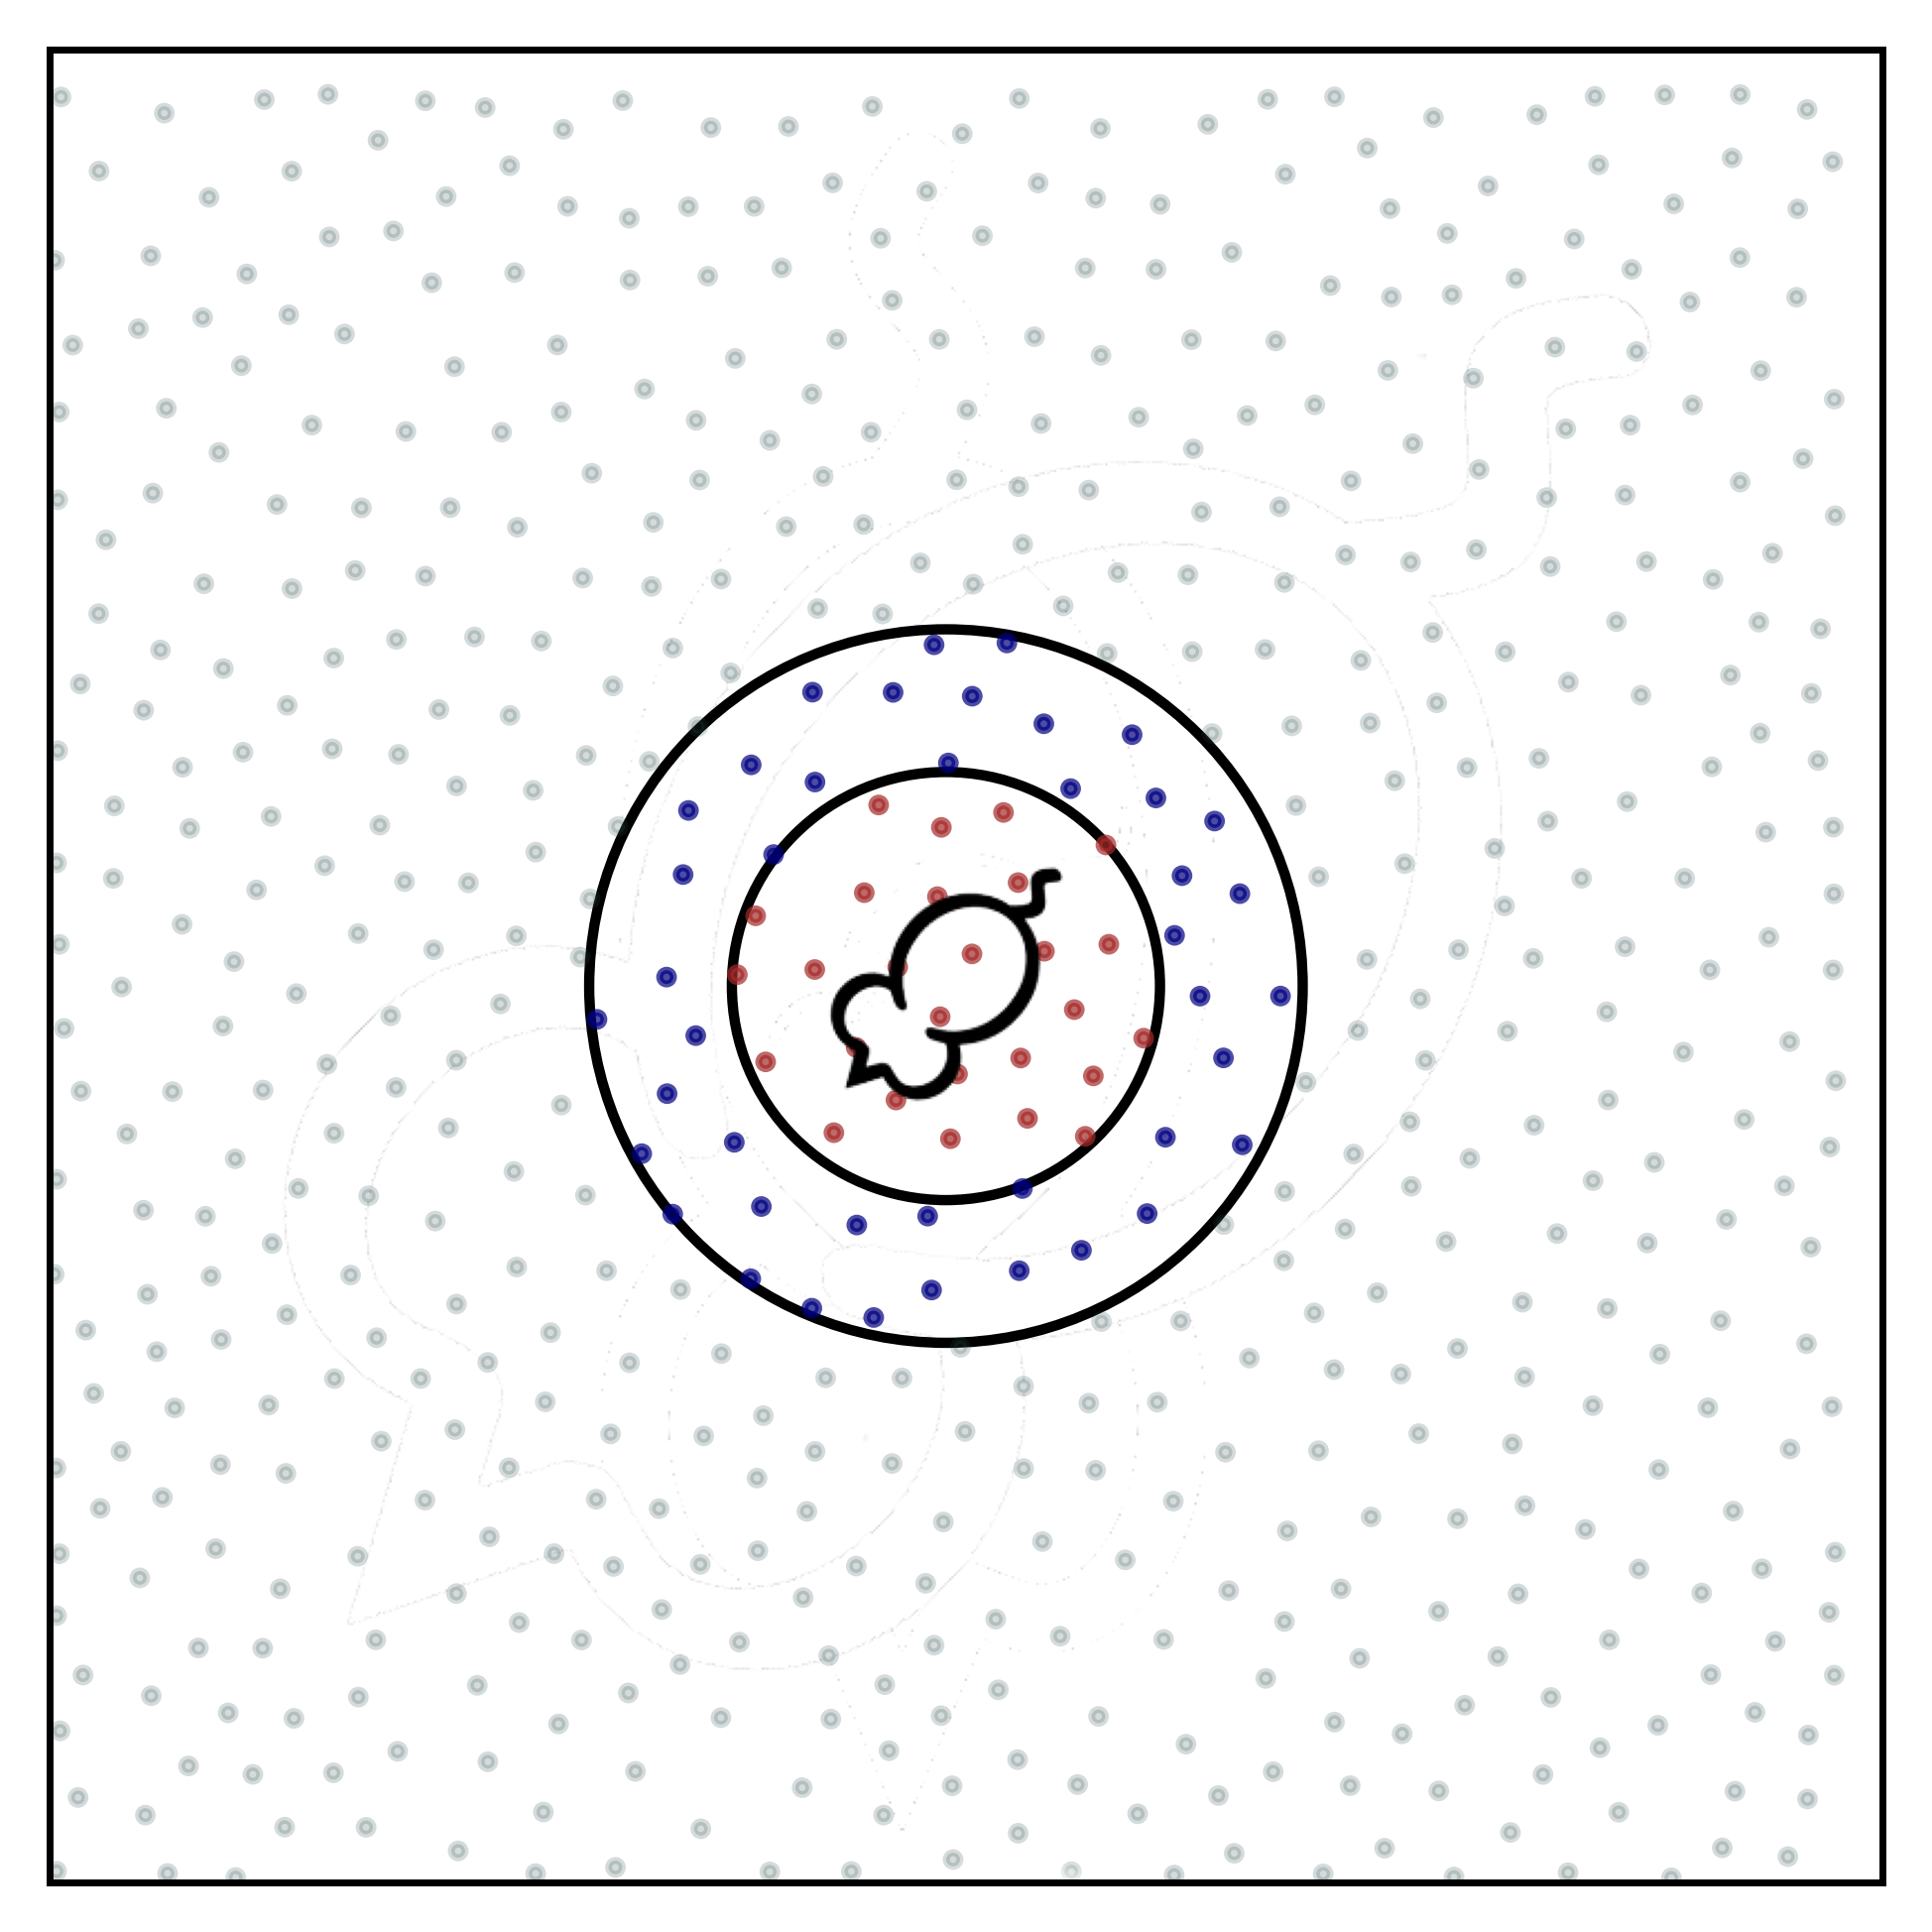
\includegraphics[width=\textwidth]{mouse_plot.png}
        \end{minipage}
        \begin{minipage}[b]{0.38\textwidth}
            \centering
            \begin{subfigure}{\textwidth}
                \subcaption{}
                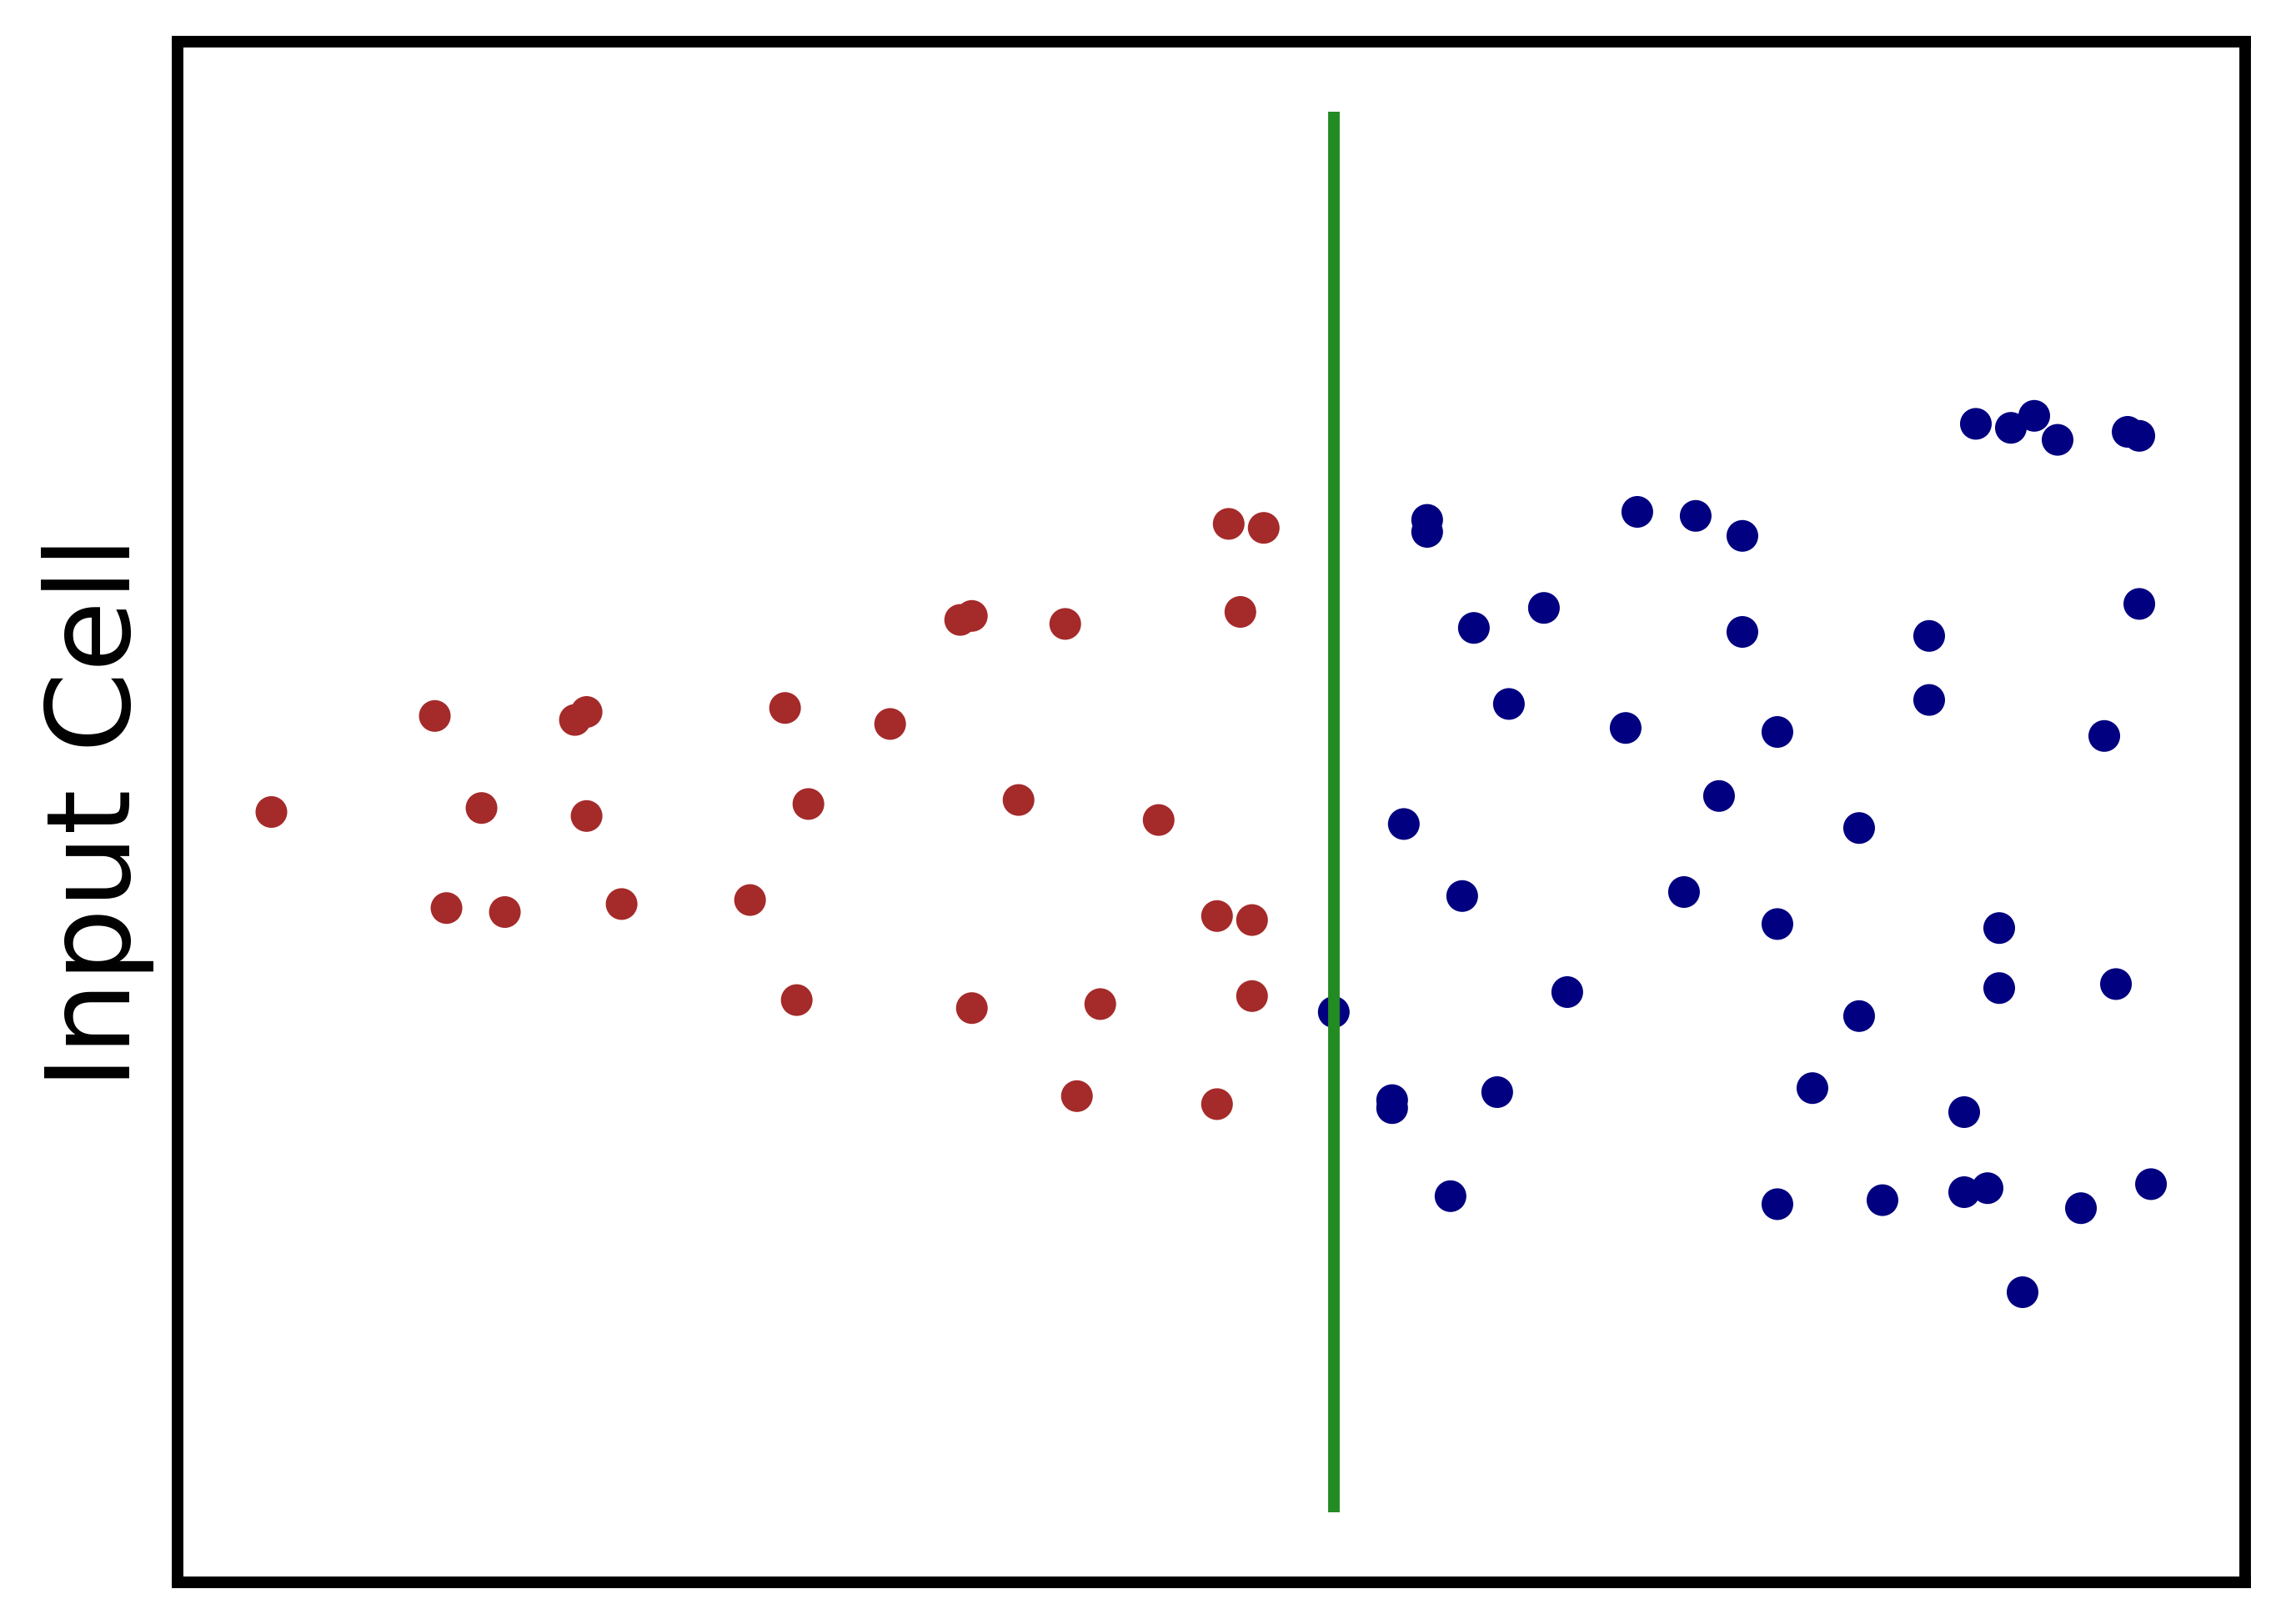
\includegraphics[width=0.95\textwidth]{input_STDP_plot.png}
            \end{subfigure}
            
            % \medskip
            
            \begin{subfigure}{\textwidth}
                \subcaption{}
                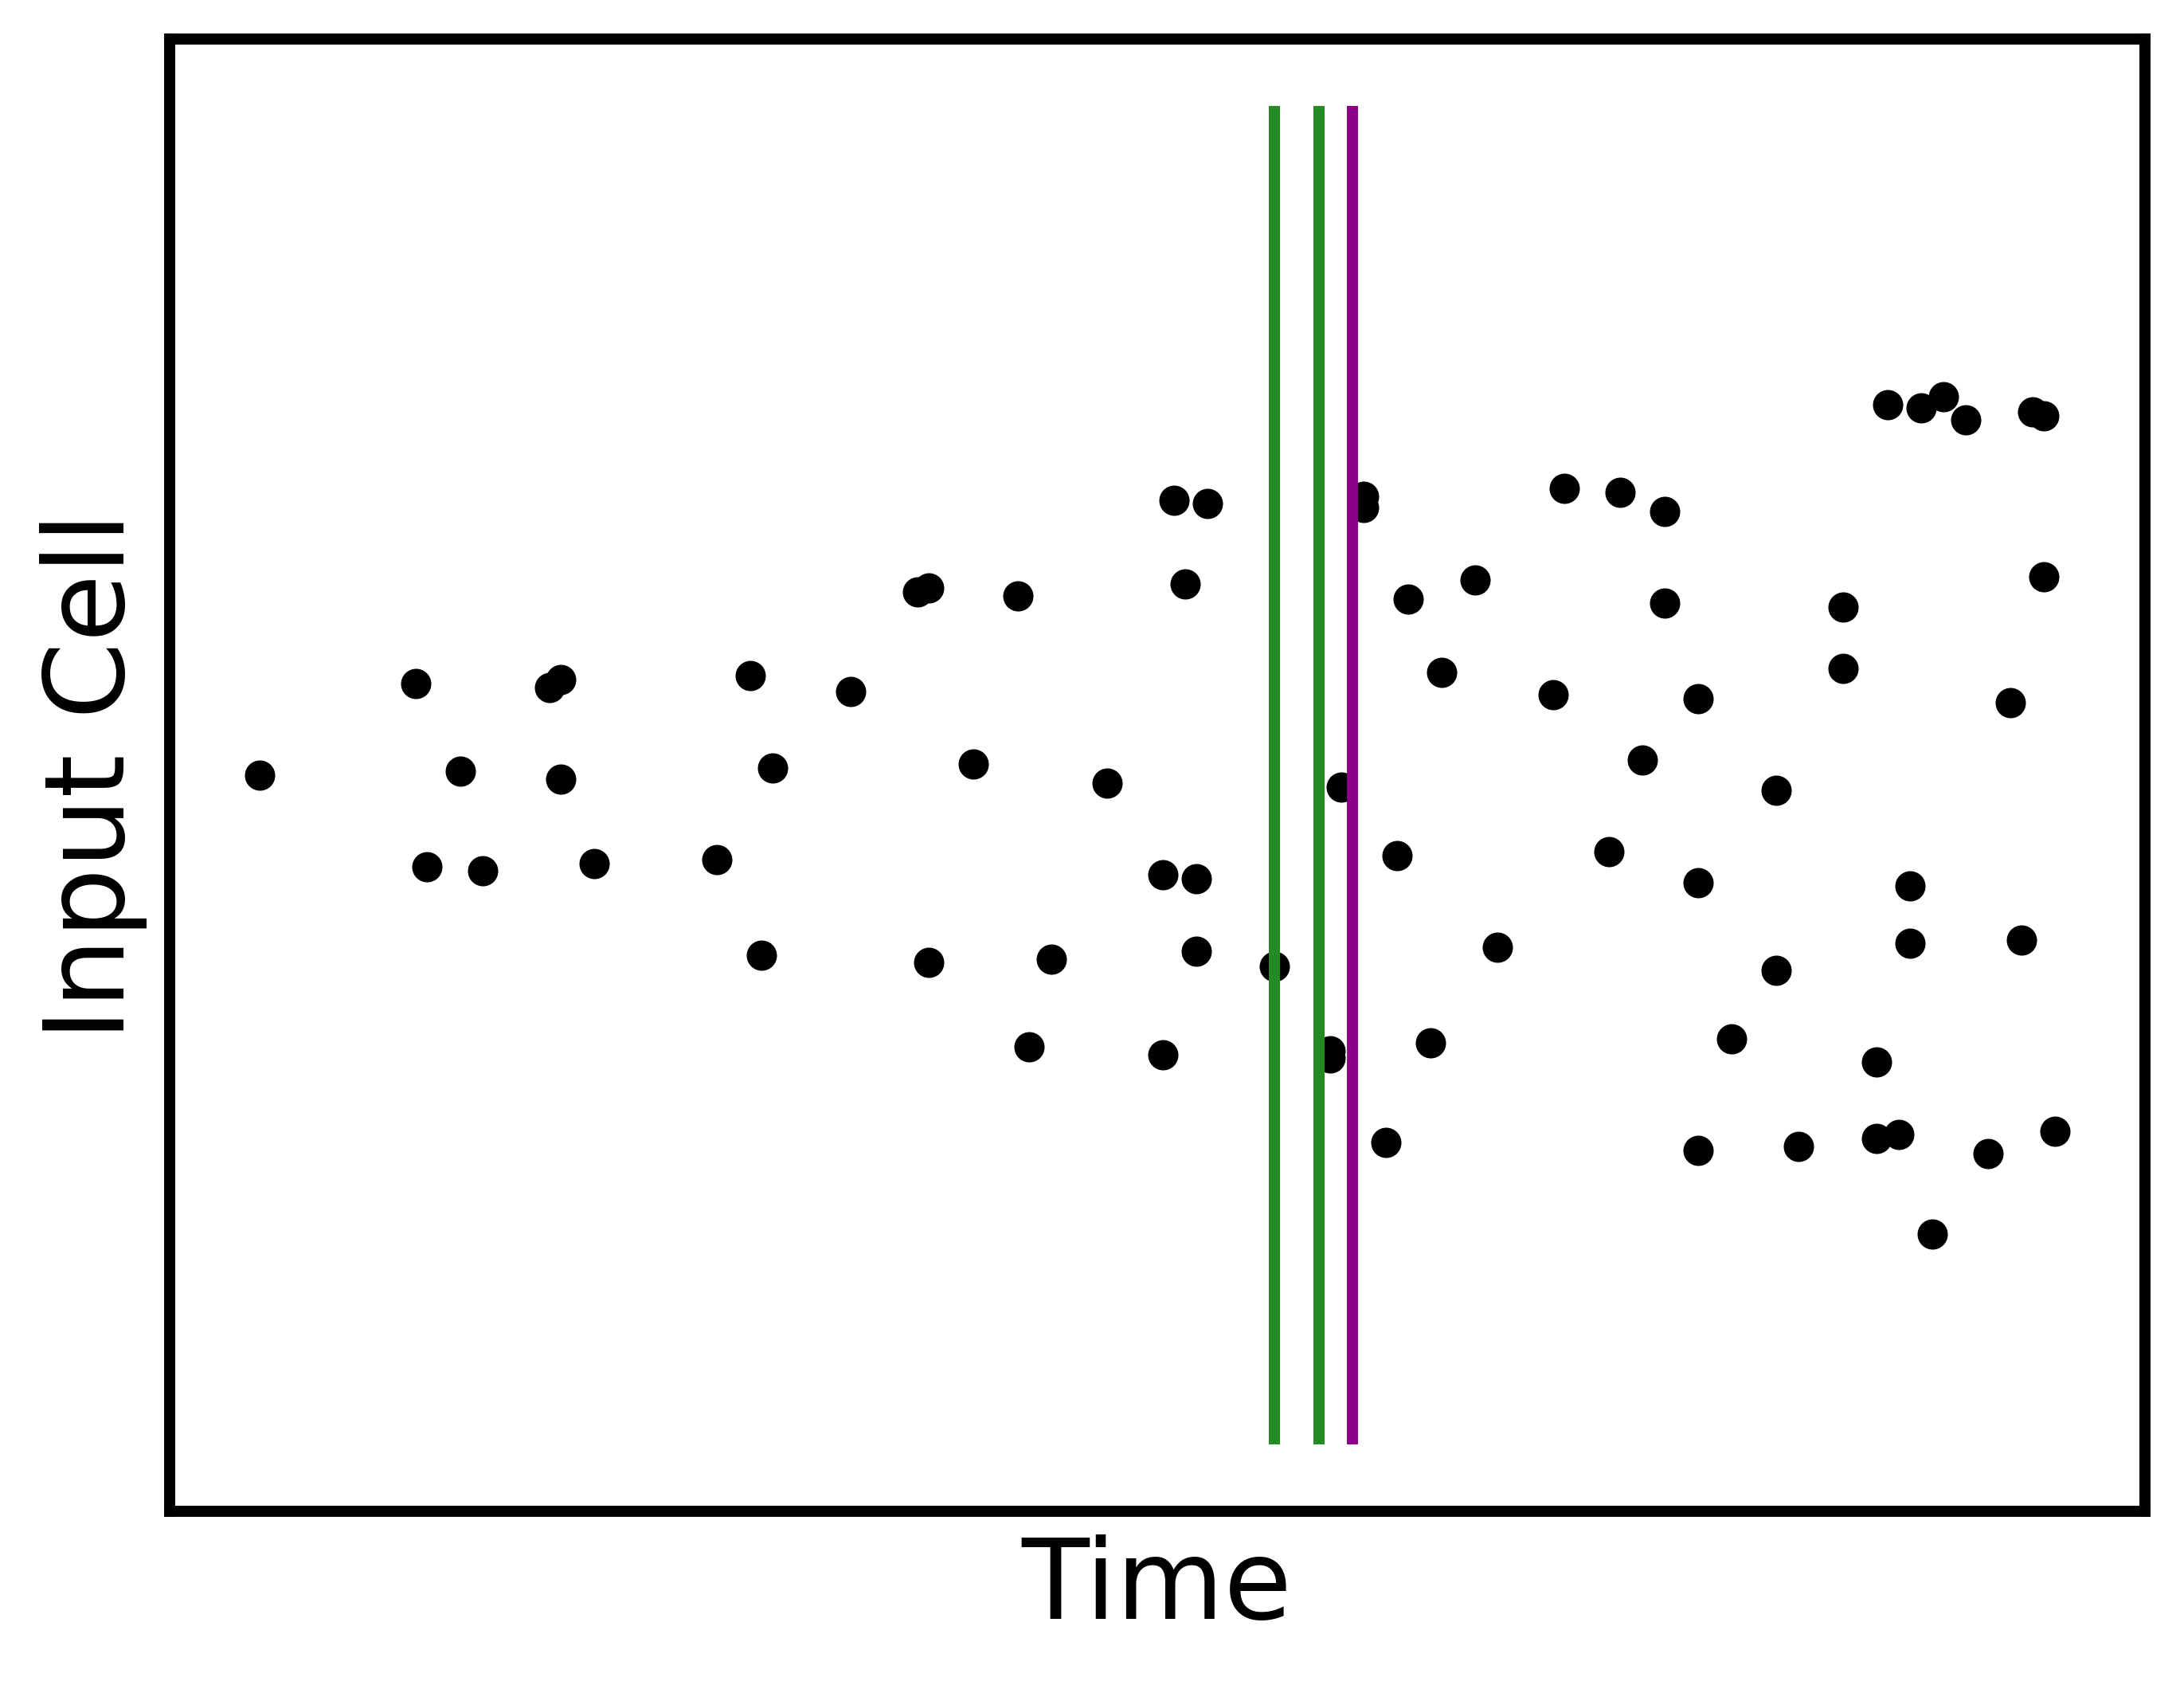
\includegraphics[width=0.95\textwidth]{input_inhibit_plot.png}
            \end{subfigure}
        \end{minipage}%
        
        \caption{The nature of phase coded spatial inputs. (a) Spatial inputs from a region surrounding the mouse will be activated each theta-cycle (10 Hz), here indicated by points within the two surrounding circles. This input is phase-coded, so cells responding to locations closest to the mouse will activate first. (b) Hypothetical raster plot showing input activity in one theta cycle. The spike time of a transition cell spike (green vertical line) determines which inputs the transition cell will associate to and dissociate from. In this case, the transition cell associates to the inputs colored red (left of the vertical line), and dissociate from the inputs colored blue (right of the vertical line). Comparing to the input's locations in (a) (color coding preserved), this becomes a center-surround learning rule. (c) Delayed inhibition (purple vertical line, rightmost) can allow multiple transition cells (green vertical lines, middle and left) to fire during the same theta-cycle.}
        
        \label{mouse_plot}
    \end{figure}

    An inhibitory layer connects transition cells laterally, causing strong inhibition, but on a delay. This leaves a narrow window in which multiple transition cells can fire, followed by complete inhibition, so some transition cells partially associate to the same areas (Figure \ref{mouse_plot} c).

    \subsection{Considering BVC inputs} \label{Considering BVC inputs}

    One goal of this work was to obtain grid cell-like transition cells with BVC inputs, and the simplest way to do this is with a direct connection between the two, so transition cell activity is based on linear summation of BVC inputs. There are reasons to think that such a network is difficult to achieve. The following idea explains this: in square environments, one could imagine picking two locations that the transition cell has associated to, denoted \((x_1, y_1)\) and \((x_2, y_2)\), and that should make up two firing fields in the hexagonal pattern. In locations \((x_1, y_2)\) and \((x_2, y_1)\), the input would be highly similar to half the input from position 1 and half the input from position 2, due to the nature of BVCs. Notably, though, the transition cell should not fire in these locations, because that would lead to rectangular grid firing patterns, not hexagonal. This would be true for all pairs of firing fields that are not parallel to one of the walls. In other words, square environments and linear summation of BVC inputs encourage rectangular fields, not hexagonal.
    
    It should be noted here that the spiking neural network itself implies non-linear features that might have enabled such a network to produce grid-cells. One way to achieve this would be with other transition cells that are sufficiently active in location \((x_1, y_2)\) and \((x_2, y_1)\), so they inhibit the first transition cell. However, due to the fine-tuning such a network would require, this network structure was not pursued further.

    An interesting alternative, which highlights an advantage of biological neurons over simplified artificial ones, appears after considering nonlinear dendritic computation on transition cells in a multi compartment model. With this in mind, although boundary vector cells technically synapse onto transition cells directly, the simulation treats dendrites as separate units within one transition cell. Each dendrite would get inputs from some subset of BVCs, and the transition cell can associate and dissociate to all inputs on an entire dendrite. Similarly to the BVC-model \parencite{Barry2006}, each dendrite would preferably be active in only single locations in the environment. This could be achieved by for instance responding non-linearly to BVC-inputs with a soft-max activation function. In the example above, this would let the transition cell associate to dendrites responding highly to \((x_1, y_1)\) or \((x_2, y_2)\), while remaining dissociated from dendrites activated in \((x_1, y_2)\) or \((x_2, y_1)\), without sacrificing biological plausibility. This multi compartment model is in line with the ideal model described in section \ref{Overall Method}.

    However, to shorten simulation time and reduce complexity, this kind of network can be simplified. This can be done incrementally, in which each step simplifies complexity but also reduces plausibility:
    \begin{enumerate}
        \item The BVC-model showed that place-like activity can be produced from BVC-inputs. As such, BVC-input can be replaced by place-like inputs directly as non-spiking dendrites in the multi-compartment model. 
        \item To reduce the number of neurons, each dendrite can connect to each grid-cell, and the dendrites can be spiking to reduce computational time for each of them. Here, the dendrites still fire in random places, according to some distribution.
        \item The dendrites can respond to places distributed in a regular, rectangular grid.
    \end{enumerate}
 
    Note that step 3 is highly similar to the already existing simulations by Waniek (citation?), just here in a spiking neural network. This was useful, because it allowed testing the hypothesis that transition cells can produce grid-like behavior in networks of more than three neurons if the inhibition is delayed, not showed in previous simulations. Then, networks could gradually be made more complex and biologically plausible, leading to a series of networks that could be tested sequentially from simple and less plausible to more complex and more plausible. The concrete implementation of each network and other considerations are treated in their own upcoming subsections.

    \subsection{Rectangularly spaced inputs} \label{Rect input}
    This network structure carries significance in this work for two reasons: it is closely related to previous TSS-simulations, and is an ideal place to investigate if larger networks still give gridness. Moreover, as outlined in section \ref{Considering BVC inputs}, it provides a useful stepping stone to subsequent models.
    
    The network has three main layers: input neurons, transition cells and inhibitory neurons. The input neurons have a preferred spatial location, and have the chance of being activated each theta cycle, which is set to happen with a 10 Hz frequency. The activation function for input neuron \(i\) with position \((x_i, y_i)\) is given in equation \ref{key1}. \begin{equation} \label{key1} delay = \frac{\sqrt{(x_i - x)^2 + (y_i - y)^2}}{\sigma} + \mu\end{equation}
    Here, x and y is the current location, \(\sigma\) is a scale parameter determining the width of input, \(\mu\) is noise and delay ends up in ms. Typically, there was a cutoff at 20 ms, so only reasonably active inputs would activate, but this cutoff was arbitrary, and could for instance depend on the transition cell scale. In this model, inputs would be distributed in a rectangular, even grid across the environment.
    
    Each of these inputs synapsed on each transition cell, with weights initialized randomly from a uniform distribution, between 0 and some maximum, \(w_{max}\). The transition cell had a voltage parameter which triggered spikes if it surpassed a treshhold, or updated according to \ref{key2}. \begin{equation} \label{key2} v(t+1) =  \begin{cases} 0, & \text{if } v(t) > \text{threshold or refractory}\\ v(t) - e^{-(v(t)) / \tau} + \sum_{0}^{i} (w_{i} \cdot i(t-delay)), & \text{otherwise} \end{cases} \end{equation}
    
    Here, v(t) is the voltage of time, \(\tau\) is a decay parameter, \(w_{i}\) is the weight of the ith input and \(i(t-delay)\) is 1 iff input i spiked at time \(t-delay\), in which time is the input delay.

    The STDP learning rule was implemented by separating potentiation and depression: upon transition cell firing, potentiation for weight \(i\) would increment dependent on presynaptic activity (\ref{key3}).  \begin{equation} \label{key3} w_i = clip(w_i + a^{pre}_i \cdot \nu, 0, w_{max})\end{equation} in which \(a^{pre}_i\) is a variable incremented when input \(i\) fires, and decays with time. \(\nu\) is here a learning rate, which can be constant or modulated by animal velocity. 
    Similarly, upon presynaptic input from input \(i\), weights are depressed if the input arrives after transition cell spike. Regardless of transition cell activity, the input weight would alse increase according to a baseline parameter. Both of these rules are captured in equation \ref{key4} \begin{equation} \label{key4} w_i = clip(w_i + (a^{post}_i + \alpha \cdot (w_{max}-w_i)) \cdot \nu, 0, w_{max})\end{equation} where \(a^{post}_i\) is a symmetric parameter to \(a^{pre}_i\), but which decrements upon post synaptic firing and decays at a separate rate. \(\alpha\) determines the magnitude of baseline weight increase.

    Transition cells then interacted by activating inhibitory neurons which inhibit all transition cells for a time, working by reducing their voltage by a large, constant amount, but which was small enough so the voltage returns to zero by the next theta by equation \ref{key2}. This inhibition was global and uniform, so each transition cell inhibited all the others and itself equally. Although this inhibition was thought to work with a delay, some simulations tried running without. In these, the delay was at the simulation software's minimum, 0.2 ms. The number of transition cells in a simulation was arbitrary, but typical values chosen were 13, 23 or 37.

    \subsection{Randomly spaced inputs} \label{Rand input}
    This network structure had similar structure and learning rule to the network in section \ref{Rect input}. In these networks, however, there was some randomness in determining which area an input neuron responded to. This was specifically done to investigate if rectangular inputs were a necessary component in developing gridness.
    
    This was tested with two separate input distributions, in addition to the rectangular grid given in section \ref{Rect input} (figure \ref{input_distribution}): One, the inputs were distributed in a blue noise like pattern, to ensure a relatively even, although not regular, distribution of spatial firing. Two, the inputs were distributed in a white noise like pattern, in which one input neuron would respond to areas independently of other areas.
    Considering the multi-compartment dendrite model mentioned previously, a white noise pattern might be most natural, because it meant that each input receptive field can be placed independently of other fields. However, it has the disadvantage that some regions in the environment will be more or less densely covered by inputs, so a transition cell that's supposed to fire in some region according to its grid might not receive any dendritic input there at all. Blue noise, which broadly speaking places the location of each spatial input as far away from every other inputs as possible, with a random element, will provide approximately even coverage of the environment.

    \begin{figure}
        \centering
        \begin{minipage}[t]{1\textwidth}
            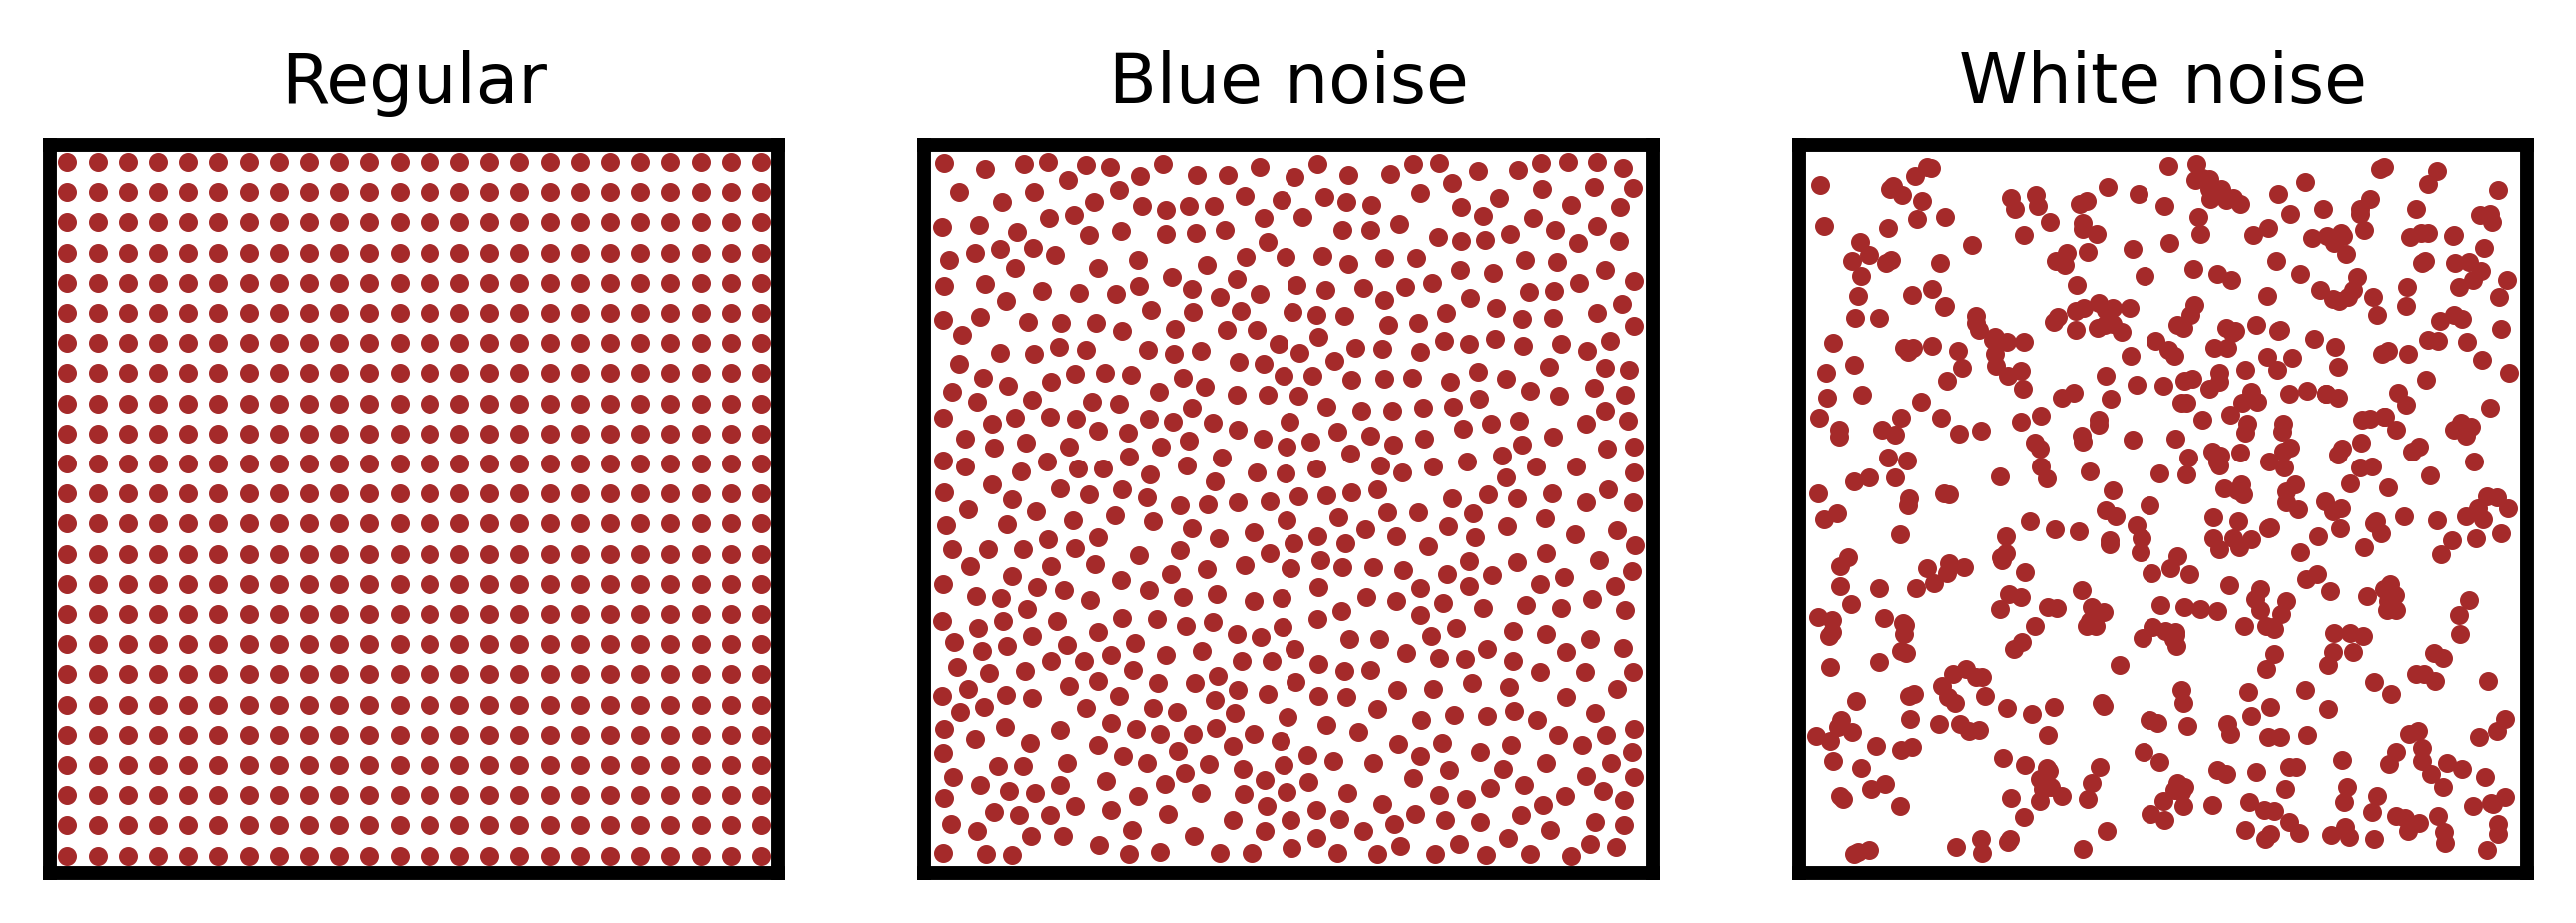
\includegraphics[width=\textwidth]{distribution_plot.png}
        \end{minipage}
        \caption{Examples of the three kinds of input distributions. Each plot shows 24x24 inputs. Regular distribution places inputs evenly across the entire environment in a rectangular way. A blue noise distribution places inputs sequentially so each is placed as far away from previously placed inputs as possible, resulting in an even, unstructured distribution. White noise distribution places inputs randomly, and independent of all other inputs, so some locations produce more input activity than others.}
        \label{input_distribution}
    \end{figure}
    
    The blue noise inputs was generated by iteratively suggesting a number of uniformly distributed points, adding the point that was the furthest from all previously added points to the added points, and repeating until the desired number of added points was reached. To allow for good spreads, the number of suggested points was directly proportional the number of existing points.
    White noise inputs were generated by getting the desired number of uniformly distributed points independently of each other.

    \subsection{Multi Compartment Model} \label{MC Model}
    A multi compartment model was briefly justified earlier, as a way to include non-linear dendritic computations which were interesting for BVC-inputs. The most natural way to implement this in the simulation software used was as a separate, non-spiking layer between the input-layer and the transition cell layer, and simulate the synapses from dendrites to transition cells as gap junctions. Although this was thought to take BVCs as inputs, an intermediary step would be to keep place-like inputs, but see how transition cells developed with this non-spiking intermediary dendrite layer.

    To justify the two-layer neuron model with dendrites and soma as a multicompartment model, the dendrites had the following properties: they only synapsed onto a single transition cell bodies, were non-spiking, and the dendrite-to-soma connectivity was modelled as a gap junction, as in (reference). In this model, each dendrite only received input from a single input neuron, to simulate the place-oriented dendrite. Each dendrite had a voltage-parameter that would increment by a factor \(w\) when receiving inputs, and decaying to 0 over time (equation \ref{key5}):
        \begin{equation}\label{key5} v_{den}(t + 1) = v_{den}(t) + e^{-(v_{den}(t))/\tau} + \sum_{0}^{i} (w \cdot i(t-delay)) \end{equation}
    
    This resembles \ref{key2}, but does not have the option of setting voltage to 0 above some threshold, as the dendrite is non-spiking. In terms of inputs, with place-based inputs, each dendrite would only receive input from one input neuron. The weight \(w\) would be a hyperparameter, not changing during a simulation, and was equal for all dendrites.
    
    Based on this, the grid cell's voltage was determined by the following equation \ref{key6}. 
        \begin{equation}\label{key6} v_{soma}(t + 1) = \begin{cases} 0, & \text{if } v_{soma}(t) > \text{threshold or refractory}\\
        \sum_{i}^{} c_i \cdot tanh(v_i), & \text{otherwise} \end{cases}\end{equation} 
        
    Here, the nonlinear function \(tanh(v_i)\) gives the dendrite a softmax-like behavior, so the dendrite at anytime is either activated or not, dependent only on its internal voltage-parameter. \(v_i\) is the voltage of dendrite \(i\), \(c_i\) is the corresponding dendrite conductance, reflecting how effectively the dendrite's voltage affects the grid cell voltage. The learning rules \ref*{key3} and \ref*{key4} is here learning over conductances instead of synapse weights, but is otherwise identical.

    With this network structure, simulation times were significantly higher than with direct connection between input cells and transition cells, because the number of dendrites was the product of the number of input cells and the number of transition cells. This limited the amount of time spent on this and subsequent models.

    \subsection{Boundary vector cell inputs} \label{BVC Model}
    This network structure was designed to be as biologically plausible as possible, but it builds directly on section \ref{MC Model}. Similarly to the model described above, inputs would synapse on an intermediary layer of dendrites, which would activate according to a softmax - function, which in turn would influence the spiking of the transition cell. Each dendrite would receive some subset of BVC-inputs, and the softmax function would be tuned so receiving only one or a few inputs would not ellicit any dendrite activity.

    From observations with different input distributions, there were reasons to think dendrites would respond to single locations, and in which the collective dendritic tree would respond evenly across the environment, such as with regular or blue noise-based input distribution. One way to do this would be by having dendrites receive a superfluous number of BVCs, and during exploration associate to some number of these so the dendrite would only respond to some location, while having dendrites avoiding to associate to the same area. However, this was not pursued further due to significant complications.
    
    Instead, a simplified version was used, in which BVCs responded preferentially to one of only two directions: north and east, with a series of different distances. Then, each dendrite received a pair of inputs, one from north and one from east, and the BVCs were carefully paired to give the dendritic tree an evenly spaced, rectangular input field. The activation function for a BVC was simply the distance to the wall in the preferred direction, converted linearly to temporal delay.
        
    The multicompartment model was a modified version of the one in section \ref{MC Model}. While dendritic voltage was the same (equation \ref{key5}), the softmax-function was here replaced with a hard step-function to simplify simulation times (equation \ref{key7}):
    \begin{equation}\label{key7} v_{soma}(t + 1) = \begin{cases} 0, & \text{if } v_{soma}(t) > \text{threshold or refractory}\\
        \sum_{i}^{} c_i \cdot (v_i > v_{threshold}), & \text{otherwise} \end{cases}\end{equation} 
    
    This is similar to equation \ref{key6}, but the dendritic conductance \(c_i\) is multiplied by a boolean which is 1 only for voltages above a threshold, \(v_{theshold}\). Considering that each dendrite only received two BVC inputs, \(v_{threshold}\) was typically between 1.2 and 1.5 times the BVC-to-dendrite weight.

    This also necessitated a change in the STDP-learning rule, since \(a_{pre}\) would increment not when the dendrite received an input, but when it passed the threshold \(v_{threshold}\).

    This model is designed to almost forcibly turn BVC-inputs into a model that resembles the first model described in section \ref{Rect input}: rectangular inputs by carefully pairing orthogonal BVCs on dendrites, and a dendritic model that has replaced a soft-max learning rule with a step-function. Despite these simplifications, which might be justified as a proof of concept for BVC-inputs, this model did not yield gridlike transition cells like the previous models, so further exploration was halted.

    \subsection{Other network models} \label{Other Models}

    A few other network structures were tried apart from the methods above, but were not explored further because they didn't produce the wanted model dynamics. This section will describe the incentives behind these structures, and how they work.

    \subsubsection{Rate coded inputs} \label{Rate input}
    One structure was designed as an alternative to using phase-coded inputs. The model still relied on dense inputs, so in each position numerous inputs would be active, but their activity was rate-coded. In the spiking neural networks simulated, neurons would always normalize to some base-voltage without external influence, and this model made rate-coded inputs by setting base-voltage depending on animal position. For relevant spatial inputs, the base-voltage would end up above threshold, leading to spiking dynamics. Very active neurons would reach this threshold faster, because the base-voltage would be significantly above threshold.

    For a rate-code like this, a transition cell would provide a feedback-signal to the input layer after spiking, which would be weak, only activating almost-active input cells at that time. Coupled with a STDP learning rule, this network structure allowed transition cells to activate the surround-inputs themselves, which would force a post-pre spike timing, leading to dissociation. A challenge with this model was keeping the input structure stable, so there would be some gap between the surround-input activation and the next round of center-inputs. However, with single-cell networks, some measure of center-surround fields was achieved, so the model might technically be viable.

    This network structure was abandoned because having feedback-connectivity from transition cells to input cells would have unwanted implications for the TSS-model as a whole, giving the transition cells sway over input activity.

    \subsubsection{Linear Summation BVC model} \label{LinnSummBVC}
    
    The simplest model with BVC-inputs to transition cells would use transition cells as simple LIF-neurons, integrating BVC-inputs and learning directly on the weights from these. Motivation for why this model was abandoned was given earlier, but this model was tested briefly nonetheless. One way to test the stability of the model was to artificially initiate the network with optimal weights, and see if it maintained the necessary firing dynamics. This was done by reverse-engineering weights, creating ideal firing patterns for each transition cell. Then, weights were set by iterating over a 48 x 48 grid of the environment and increasing weights from inputs relevant to a firing position, decreasing weights from inputs that were irrelevant. This approach was not tried for any other methods, but when it failed to give the wanted spiking dynamics in the network, along with the arguments presented in section \ref{Considering BVC inputs}, this approach was abandoned.

    \subsubsection{Linear Multi-compartment Models} \label{Lin MCModel}

    Models described in section \ref{MC Model} used a multi-compartment model of the neuron to allow dendritic computation to convert vector-based inputs to place-like inputs the transition cell could learn transitions on. In those models, the voltage in a dendrite is transformed to a voltage in the transition cell body through a nonlinear softmax-function, but using a linear convertion was also tried. In this model, the transition cell body voltage was the sum of all dendrite voltages multiplied by conductances: \begin{equation}\label{key8} v_{soma}(t + 1) = \begin{cases} 0, & \text{if } v_{soma}(t) > \text{threshold or refractory}\\
        \sum_{i}^{} c_i \cdot v_i, & \text{otherwise} \end{cases}\end{equation} 
    This model was discarded for not showing the necessary dynamics: with BVC-inputs, a number of dendrites were slightly active in a lot of locations, participating in transition cell activity. Even if the learning rules were thresholded, so the STDP- and baseline-learning rules would only apply to moderately active dendrites, this errant activity would mean transition cells would activate in too many consecutive locations, losing circular firing fields.

    \subsection{Simulation software} \label{Sim software}
    
    All models and implementations can be found on github(Insert link here?), and while the simulation data is not available on github due to storage capacity, it is available (somewhere else?). All simulations were implemented in python, using the Brian2-library for its flexibility and easy implementation \parencite{Brian2}. With this framework, setting up simulations was straight forward, and allowed time-improvements such as only updating STDP-variables when relevant events occurred, not at every time step. Time steps were typically at 0.1 ms, which was also the minimal synaptic delay.
    
    Simulations with place-inputs used self-written simulated trajectories, simulated with 10 ms time steps and a square environment. Position was treated like a continuous variable, with velocity and rotational velocity determined by normal distributions from one time step to the next. In simulations using boundary vectors, the external RatInABox library was used \parencite{RatInABox}. 
    
    From the trajectories, spatial inputs were calculated prior to simulations, using either position- or boundary information, and added to a brian2 spikeGeneratorGroup. The network state and weights was stored frequently during simulations.

    \subsection{Analysis} \label{Analysis}
    To investigate the firing properties of the network of transition cells, weights were frozen, and the activity of the network was sampled from each position in an even 48 x 48 grid across the environment. In simulations with noise, each position was sampled 5 times, while they were sampled only once without noise. This gave momentary pictures of the network state, which were subsequently stored as spike trains and then converted to histograms of spatial firing fields. Due to the time in took to get one sample, each simulation was typically sampled each 5 minutes of simulation time.

    Five primary variables were derived from each simulation: gridness score, spacing, orientation, phase distribution and temporal stability.
    
    The measure used to evaluate the hexagonality of the transition cells was primarily the gridness score. To find this score, an annulus was extracted around the center of the autocorrelation of the spatial firing fields of a sample. The size of this annulus was estimated to find the first ring of maxima around the center. Using this annulus, gridness score was determined as \[gscore = min(a_{60\degree}, a_{120\degree}) - max(a_{30\degree}, a_{90\degree}, a_{150\degree})\] in which \(a_{n\degree}\) is the correlation between the annulus and itself rotated \(n\) degrees.

    Gridness spacing was found by evaluating the gridness score with multiple estimations of annulus size, and determining values that gave the highest score. Because of the discretization of space, multiple spacings would give similar scores, in which the mean was taken.

    Orientation was determined only in cells with a positive gridness score. Orientation was determined as the angle between the horizontal line and the first maxima within the annulus, extracted similarly to in the gridness score.

    Phase distribution was only evaluated for cells with positive gridness and an orientation between \(-5\degree\) and \(5\degree\), as this seemed to be dominant for most simulations. In simulations with multiple cells passing these criteria, one cell was chosen at random as a basis for comparison. All other cells would be evaluated relative to this basis by doing a cross correlation, and finding the maximal value. To find all positions relative to the rhombus, the phase-difference was unsheared, so the rhombus would be a rectangle. Then, phase differences could be reduced to the within the rectangle by a modulo-operation, and sheared again to be placed within the rhombus.
    
    Temporal stability was estimated by getting the variance in pixel-values in spike plots across time for each cell in the latter half of a simulation, and comparing the mean variances to the mean variance of shuffled pixel values. This approach was enabled by the sampling scheme, in which each location in the environment was sampled equally at even time points. Shuffling the spike plots represented the expected temporal stability if there would be no correlation from one timepoint to the next, while a lower variance would imply a positive correlation of firing fields from one time to the next. [add a figure to show this, as well as other features?]


    \section{Results} \label{Results}

    \subsection{Defining Typical Parameters: a Standard Model} \label{Standard model}
    A few models were tested in this work. In most of these, overall network structure was kept the same, varying instead on certain parameters that were perceived as critical: the distribution of inputs, inhibition delay, the number of transition cells in a network and the role of noise in the spatial inputs. In addition to these variants, this section will show results from a multi-compartment model with non-spiking dendrites, both with place-like inputs and boundary vector cell inputs. Most hyperparameters were not tested, or not tested thoroughly, for reasons related to time constraints. In that light, this section will describe typical parameters of one model, and some of the considerations made in setting some of the parameters. This set of typical parameters ends up making out a standard model, which will be used as a baseline for comparison in the rest of the article. This model was chosen as the base model for comparison because it is closest to previous simulations of the models run in this work.

    Table \ref{param_table} shows a typical set of hyperparameters, partially chosen to be biologically plausible, but some sets of parameters were calibrated in order to achieve a wanted dynamic. Since the input was phase-coded relative to theta, weights and spiking threshold were set so the first transition cell would spike typically about halfway between the first input and the phase-delay cutoff. This was thought to encourage even center- surround fields under a STDP learning rule. Inhibitory delay was set to give a brief window for other cells to fire, and is probably shorter than expected biologically [source?]. The apost, apre and baseline was set up to work in conjunction so potentiation and depression would approximately balance each other out, according to equations \ref{key3} and \ref{key4}. This model also assumed zero noise in the phase delay for simplicity, but different levels of noise was tested in different models.

    \begin{table}[H]
        \caption{Example parameters for simulations. The parameters are partially chosen for biological plausibility, and partly adapted to achieve desired firing dynamics.}
        \begin{tblr}
            {
            colspec = {X[c,h]X[c]},
            stretch = 0,
            rowsep = 6pt,
            hlines = {black, 1pt},
            vlines = {black, 1pt},
        }
        
            \textbf{Parameter} & \textbf{Value} \\
            \# Transition cells & 13\\
            \# Inputs & 576 (24x24) \\
            Theta rate & 10 Hz \\
            Phase-delay cutoff & 20 ms \\
            \(\sigma\) & 0.012 \\
            \(\mu\) & 0 \\
            Transition cell threshold & 1.0 \\
            Transition cell \(\tau\) & 10 ms \\
            \(w_{max}\) & 0.14 \\
            \(w_{init}\) & uniform[0-0.75 \(\cdot w_{max}\)] \\
            \(A_{pre}\) & 0.01 \\
            \(A_{post}\) & -0.007 \\
            \(\tau_{pre}\) & 8 ms \\
            \(\tau_{post}\) & 80 ms \\
            Baseline & 0.005 \\
            Inhibitory delay & 0.6 ms \\
        \end{tblr}
        \label{param_table}
    \end{table}

    The simulations were run on a simulated trajectory, as described in the methods, using a one meter by one meter square environment. While weights and parameters were stored mid-simulations, data was also extracted from each model by sampling each position in a grid after freezing learning. For a network with parameters from table \ref{param_table}, typical spike plots are shown in figure \ref{reg_spike}. 
    
    
    \begin{figure}[htbp]
        \centering
        \includegraphics[width = \linewidth]{reg/spike.png}
        \caption{Sampled activity from seven transition cells in the same network throughout a simulation. Each plot represents activity in the same 1 x 1 m environment, subdivided into a 48 x 48 grid in which each position was sampled for a single theta cycle. Learning was disabled during sampling. Bright spots in the plots represent locations in which a transition cell was active, and each plot is smoothed with a gaussian filter. This sampling method is used for all models, although the number of samplings per position depended on noise levels.}
        \label{reg_spike}
    \end{figure}
    
    Clearly, transition cells typically develop center-surround fields quickly, evidenced already after 5 minutes of exploration from random initial activity patterns. Looking at the temporal development of spike plots, while it seems like firing fields are somewhat stable in time, the development of hexagonal gridness is gradual.

    Five primary variables were quantified about transition cell activity, all using these spike plots. The primary one is gridness score, which quantifies the degree to which the firing fields are hexagonal. One caveat of the grid score is that it is highly sensitive to shearing and rectangular patterns, so transition cells with distinct periodic firing fields, but without strict hexagonality, can have highly negative grid scores.
    
    The three primary variables for looking at grid cell populations was also used for these transition cells: grid spacing, orientation and phases. 
    
    Finally, a measure of temporal stability says something about whether the network converges to some state or is shifting. 
    
    The following sections will outline results according to these five parameters for ten models: A standard model with parameters outlined in table \ref{param_table}, two models with similar parameters but different spatial input distributions (blue noise and white noise distributions, see figure \ref{input_distribution}), networks with more transition neurons (23 and 37 cells), networks with minimal inhibitory delay (0.2 ms, but referred to as 'no delay') and networks with different levels of input noise. 
    
    Input noise occurred in the phase-delay of the input. Each theta cycle, each input had an expected delay depending on its spatial relevance relative to the animal's current position. In each model, the actual delay on an input was modelled as normally distributed around this delay, with standard deviations of 1, 2 or 4 ms. All maintained a 20 ms temporal window each theta cycle.

    In addition to these models, a multi-compartment model with parameters similar to the standard model was tested as a proof of concept, referred to as the MC Model. This model also used place-like inputs, but these inputs synapsed on non-spiking dendrites, each dendrite only receiving inputs from one input cell, and each dendrite subsequently affecting the transition cell spiking in a gap-junction-inspired way.

    \subsection{Gridness scores in the different models} \label{Gscore}
    
    The central question to this work was whether the network structure and learning rule described in the methods section could produce transition cells with a hexagonal firing patterns, which can be quantified by the gridness score. This gridness score was always computed on spike plots such as those shown in figure \ref{reg_spike}, sampled evenly across the environment with frozen weights. This was tracked in ten different network models, each simulated thirty times and sampled every five minutes across a 95-minute simulation. Figure \ref{gridness_plots} a shows final mean gridness score for each simulation, grouped by model, while figures \ref{gridness_plots} (b-e) show the temporal development of gridness scores in the ten models according to groups.
    
    \begin{figure}[htbp]
        \centering  
        \begin{minipage}[b]{1\textwidth}
            \centering
            \subcaption{}
            \includegraphics[width=\textwidth]{model_comparison/model_comparison_gscores.png}
        \end{minipage}
        \begin{minipage}[t]{1\textwidth}
            \begin{subfigure}{0.5\textwidth}
                \subcaption{}
                \includegraphics[width=0.98\textwidth]{model_comparison/line_plot0.png}
            \end{subfigure}
            \begin{subfigure}{0.5\textwidth}
                \subcaption{}
                \includegraphics[width=0.98\textwidth]{model_comparison/line_plot1.png}
            \end{subfigure}
            \begin{subfigure}{0.5\textwidth}
                \subcaption{}
                \includegraphics[width=0.98\textwidth]{model_comparison/line_plot2.png}
            \end{subfigure}
            \begin{subfigure}{0.5\textwidth}
                \subcaption{}
                \includegraphics[width=0.98\textwidth]{model_comparison/line_plot3.png}
            \end{subfigure}
        \end{minipage}
        \caption{Gridness scores for ten model types. (a) Each scatter point represents mean gridness in one simulation after 95 minutes simulation time. Bars are means across all simulations for one type. (b-e) Loosely grouping the model types into four or five main categories. Colors are maintained from (a). (b) The multi-compartment (MC) model shares important parameters with the standard model; they both have networks of 13 transition cells, no input noise and rectangularly spaced inputs. The standard model seems to outperform the MC Model, but both show clear gridness. (c) Models receiving inputs from a blue noise distribution have approximately equal gridness to the standard model, while transition cell networks receiving white-noise inputs do not seem to have the same development. (d) Transition cells exhibit clear gridness both with minimal inhibitory delay and with different network sizes. While a network of 23 transition cells see the same gridness as the standard model, 37 transition cells have a somewhat reduced gridness. Without inhibitory delay, gridness is also reduced, and less stable. (e) While simulations with normally distributed input noise and std 1 or 2 ms have gridness comparable to the noiseless standard model, a std of 4 ms in input noise is not as robust.}
        \label{gridness_plots}
    \end{figure}
    
    While the standard model as described here produced highest scores, multiple other models had comparable scores. Networks with blue noise-distributed inputs, or with 23 transition cells, or with 1 ms noise, had comparable final griness, and developed approximately equally quickly. The multi compartment model also had high gridness, but not comparble to the above-mentioned groups, which was also true for simulations with 37 transition cells, minimal inhibition delay or 2 ms noise. Finally, white noise inputs performed worse, while having some positive gridness, and 4 ms input noise did not produce stable hexagonality at all.
    
    Despite the differences in gridness, virtually all cells across all simulations seemed to develop clear, isolated firing fields, and fired in multiple locations across the environment. This is true when for instance looking at the firing plots of white noise inputs or minimal inhibitory delay. This reflects some inability in the learning rule to encourage tight bundling of firing fields, which is also reflected in the standard model when the baseline learning parameter is set to 0 [preliminary results, check these later](also, ref some figure here?). 

    In all models, within-simulation variance in gridness was high, and virtually all simulations had some cells with a negative gridness score at all times (figure \ref{gscore_distribution}). Low gridness scores can be explained by grid shearing or firing fields that aren't evenly distributed across the environment, while negative scores tend to reflect rectangularity. [I should probably investigate if cells with negative scores tend to have negative scores across a simulation].

    \begin{figure}[H]
        \centering
        \begin{minipage}[b]{0.95\textwidth}
            \subcaption{}
            \includegraphics[width = 0.95\linewidth]{reg/distribution.png}
        \end{minipage}
        \begin{minipage}[t]{0.95\textwidth}
            \subcaption{}
            \foreach  \filename in {
                model_comparison/distribution_blue_noise.png,
                model_comparison/distribution_white_noise.png,
                model_comparison/distribution_no_delay.png,
                model_comparison/distribution_23grid.png,
                model_comparison/distribution_37grid.png,
                model_comparison/distribution_GJ.png,
                model_comparison/distribution_1ms_noise.png,
                model_comparison/distribution_2ms_noise.png,
                model_comparison/distribution_4ms_noise.png}
            {
            \begin{subfigure}{0.323\textwidth}
                \includegraphics[width=\textwidth]{\filename}
            \end{subfigure}
            }
        \end{minipage}
        \caption{Distribution of gridness scores in the different models. (a) Standard model gridness distribution with spike plot examples. Although the mean gridness of this model is considered high (above 0.6), most simulated networks contain cells with negative or low gridness score. Negative gridness is typically produced by rectangular patterns, as shown in the two leftmost spikeplot examples. The two middle examples show activity in cells with positive, but low gridness scores. To have a gridness score above 1, the hexagonal pattern must typically span the whole environment without shearing or rectangularity. (b) Gridness score distributions for the remaining nine models.} 
        \label{gscore_distribution}
    \end{figure}

    Interestingly, the distributions of grid scores can also reflect features of models with lower gridness scores. The models with minimal inhibitory delay seem to have a wide variety in gridness, so some cells are highly gridlike and others highly un-gridlike, while models with white noise inputs have a higher mode, but rarely sees highly hexagonal cells. In the latter case, it might seem like the cells don't pack firing fields closely enough to develop high gridness, while in the former the between-transition cell competition might be too high to support large networks with high hexagonality.

    \subsection{Orientation and phase distribution} \label{OrientationPhaseResults}

    According to experimental data, grid cells in a module align in orientation with a wall-angle offset of 7.5\(\degree\), which was also observed in previous simulations of the TSS-model with related learning rules. Grid cells with similar spacing and orientation have phases that are evenly distributed on the toroidal manifold the network is active on. Here, orientation was only computed for transition cells with positive gridness, and normalized to a value between 0 and 60 \(\degree\). Phase distribution was only computed on cells that aligned with the dominant orientation of that model so phase distribution could be accumulated across multiple simulations, and normalized to position within a rhombus of the environment.

    In all simulations, the preferred orientation was around 0\(\degree\), which indicates that transition cells align firing fields preferentially parallel to one of the environment walls (ref figure). However, this wasn't a strong preference, at most one in four cells with positive gridness showed this directionality. Models with noise had less of an orientation preference, as was the case for models with no inhibitory delay. 
    
    \begin{figure}[H]
        \begin{minipage}[t]{\linewidth}
            \begin{subfigure}{0.2\textwidth}
                \includegraphics[width=\textwidth]{model_comparison/model_comparison_orientation_regular.png}
            \end{subfigure}
            \foreach \filename in {
                model_comparison/model_comparison_orientation_blue_noise.png,
                model_comparison/model_comparison_orientation_white_noise.png,
                model_comparison/model_comparison_orientation_23grid.png,
                model_comparison/model_comparison_orientation_37grid.png}
            {
            \begin{subfigure}{0.18\textwidth}
                \includegraphics[width=\textwidth]{\filename}
            \end{subfigure}
            }
            \begin{subfigure}{0.2\textwidth}
                \includegraphics[width=\textwidth]{model_comparison/model_comparison_phase_regular.png}
            \end{subfigure}
            \foreach \filename in {
                model_comparison/model_comparison_phase_blue_noise.png,
                model_comparison/model_comparison_phase_white_noise.png,
                model_comparison/model_comparison_phase_23grid.png,
                model_comparison/model_comparison_phase_37grid.png}
            {
            \begin{subfigure}{0.18\textwidth}
                \includegraphics[width=\textwidth]{\filename}
            \end{subfigure}
            }
            \vspace*{0.03\linewidth}

            \foreach  \filename in {
                model_comparison/model_comparison_orientation_no_delay.png,
                model_comparison/model_comparison_orientation_1ms_noise.png,
                model_comparison/model_comparison_orientation_2ms_noise.png,
                model_comparison/model_comparison_orientation_4ms_noise.png,
                model_comparison/model_comparison_orientation_GJ.png}
            {
            \begin{subfigure}{0.18\textwidth}
                \includegraphics[width=\textwidth]{\filename}
            \end{subfigure}
            }
            \foreach  \filename in {
                model_comparison/model_comparison_phase_no_delay.png,
                model_comparison/model_comparison_phase_1ms_noise.png,
                model_comparison/model_comparison_phase_2ms_noise.png,
                model_comparison/model_comparison_phase_4ms_noise.png,
                model_comparison/model_comparison_phase_GJ.png}
            {
            \begin{subfigure}{0.18\textwidth}
                \includegraphics[width=\textwidth]{\filename}
            \end{subfigure}
            }
        \end{minipage}
        \caption{Orientations and phases of all models. Transition cells prefer a 0 \(\degree\) orientation in most models (1st and 3rd row), exceptions being the minimal inhibitory delay model and the model with most input noise. The standard model and blue noise input distribution model seem to have the strongest preference, while either increasing network size or adding noise reduces the preference somewhat. To compute phase distributions, only transition cells with positive gridness and an orientation between -5 \(\degree\) and 5\(\degree\) were considered. Within a simulation, one of the qualifying transition cells was chosen as a reference, and the dots show the other qualifying transition cells' phase relative to their reference (rows 2 and 4). This phase was computed as the offset of the peak relative to the center in the cross correlogram between the transition cell and the reference.}
        \label{orientation_phase_plot}
        
    \end{figure}

    One thought was that simulation times were too short for transition cells to develop the 7.5\(\degree\) orientation preference seen in previous simulations, but this did not seem to be the case (add some results indicating this?).

    Phase distribution can only be investigated in simulation with minimally two cells sharing orientation, preferably more, and this was more common in larger networks. From looking at the networks with 23 or 37 transition cells, the phase distributions seem somewhat even, although the central area near the top of the rhomboid seems less populated (figure ref). Notedly, computing these phases was limited by the spatial resolution of the activity sampling, leading to rounding values.
    
    It was briefly checked if the 37-cell networks had a toroidal structure in the population activity, which would be expected for grid cells belonging to the same module. This did not yield interesting results, and while it should be not that those methods are created for larger networks, higher temporal resolution and rate-based network activity, it seems unlikely that networks with at most a third of the cells sharing orientation would have a highly ordered population activity structure.

    \subsection{Gridness spacing} \label{Spacing}

    All ten models introduced in section \ref{Standard model} used, barring noise, the same threshold for which spatial inputs would activate in a given location. Given a STDP-learning rule that lets an active transition cell decorrelate from less relevant spatial inputs, it would be expected that this relevance threshold is critical for the size of transition cell firing fields. That does not, however, mean that all models would give transition cells with the same spacing.

    \begin{figure}[h]
        \centering
        \begin{minipage}[t]{\textwidth}
            \subcaption{}
            \includegraphics[width = \textwidth]{model_comparison/model_comparison_sigmas.png}
        \end{minipage}
        \begin{minipage}[t]{\textwidth}
            {
                \begin{subfigure}{0.126\textwidth}
                    \subcaption{}
                    \includegraphics[width = \textwidth]{model_comparison/spacing_spikeplot_simspam.png}
                \end{subfigure}
            }
            \hspace*{-0.01\textwidth}
            \foreach \filename in {
            model_comparison/spacing_spikeplot_noise_sims2.png, 
            model_comparison/spacing_spikeplot_noise_sims.png, 
            model_comparison/spacing_spikeplot_noise_sims3.png}
            {
                \hspace{0.01\textwidth}
                \begin{subfigure}{0.26\textwidth}
                    \subcaption{}
                    \includegraphics[width = \textwidth]{\filename}
                \end{subfigure}
            }
        \end{minipage}
        \caption{Grid spacing across ten models. This was computed as the spacing giving maximal gridness score for each cell after 95 simulation minutes. This was then filtered for cells with positive gridness. (a) Each dot represents the spacing in a single transition cell, sorted by model. Horizontal lines are model medians: for many models, the density is significantly higher close to the median that around.  Notably, while mean spacing seems invariant on network size, adding noise seems to increase median spacing. Models with white noise inputs also had increased spacing, but that might be caused by poor gridness overall. Moreover, the multi-compartment model had higher spacing than the standard model. (b - e) Spike plots of models with identical parameters apart from input noise. (b) The standard model, without input noise, has a mean spacing of about 32.5 cm. As opposed to models with noise, transition cells can fit four firing fields horizontally in a 1 x 1 environment (lower spikeplot). (c \& d) Models with 1 ms and 2 ms input noise have approximately similar mean spacing, at about 35 cm. (e) While 4 ms noise doesn't produce high gridness or clean firing fields, the average spacing is significantly larger than other models, with mean around 50 cm.}
        \label{spacing_plot}
    \end{figure}

    Curiously, while most models had highly similar spacing, which seems independent of input distribution and size of the transition cell layer (around 10.8 cm spacings), adding noise increased spacing, and it depended on amount of noise (figure \ref{spacing_plot}). This was especially true for the highest noise level tested, with mean spacing at 50 cm, while the 1 ms and 2 ms models had an approximately 35 cm spacing preference.

    \subsection{Temporal stability} \label{TempStab}

    From earlier figures, it does seem like transition cells in many of the networks develop gridness over time, so the firing fields get more hexagonal over time. However, it is unclear if the fields converge on some stable configuration, or if they continuously shift throughout the simulation. Under the TSS model, transition cells with incremental, gradually improving hexagonality might be beneficial because transition cells also interconnect with place cells, so big changes in transition cell area will necessitate accurate changes in the connectivity between transition cells and place cells.

    
    \begin{figure}[h]
        \centering
        \begin{minipage}[t]{\textwidth}
            \subcaption{}
            \includegraphics[width = \textwidth]{model_comparison/model_comparison_temporal_stability.png}
        \end{minipage}
        \begin{minipage}[t]{\textwidth}
            \begin{subfigure}{0.347\textwidth}
                \subcaption{}
                \includegraphics[width = \textwidth]{model_comparison/sum_spikeplot_multi-grid.png}
            \end{subfigure}
            \foreach \filename in {
            model_comparison/sum_spikeplot_GJ_model.png, 
            model_comparison/sum_spikeplot_noise_sims3.png}
            {
                \hspace*{0.01\textwidth}
                \begin{subfigure}{0.297\textwidth}
                    \subcaption{}
                    \includegraphics[width = \textwidth]{\filename}
                \end{subfigure}
            }
        \end{minipage}
        \caption{Temporal stability of different models. (a) The measure used to quantify temporal variance was the mean variance in spiking activity from one sampled time to the next, normalized by the variance in the shuffled data. A one in this score would indicate that there is no linear correlation between spiking from one sample time to the next, five simulation minutes later, while values close to zero indicate a positive correlation. Input noise seems to decrease temporal stability, while inhibitory delay seems to increase it. Larger networks also seem more resistant to change. (b - d) The 95 minute sample activity (row 1) and summed activity over all sample times (row 2) for three different models. All three models seem to have single-time samples with clear regions of activity and inactivity. The summed activity, however, shows that transition cells in the 37 transition cell model and the multi compartment model have maintained firing fields over time, while the noise model has not. This is reflected in their relative temporal variance scores.}
        \label{temporal_stability_plot}
    \end{figure}

    To investigate this, a measure for temporal stability was used which tracks the transition cell activity in each of the sampled locations over time (figure \ref{temporal_stability_plot} a). The measure is a temporal correlation, in which the variance from one sample to the next, taken five simulation minutes later, is compared to the variance with shuffled data. This shuffled variance is used as a standard for no correlation, so a variance between 0 and 1 represents a positive temporal correlation, and variances above one is a negative correlation.
    
    A positive correlation is clearly expected, because the input weights at one sampling time will be correlated to input weights at the next sampling. Additionally, the STDP learning rule is expected to encourage a cell to associate to some place and keep firing there. As such, the measure doesn't clearly indicate what should be understood as high temporal stability. Figures 
    
    \ref{temporal_stability_plot} (b - d) shows activity of two cells for three different models: the 37 transition cell model, which had the highest recorded stability, the 4 ms noise model with the lowest stability and the multi compartment model as an intermediate one. The first row in each plot shows the activity at the final sampled time, 95 minutes, while the second row shows the summarized activity over all times. The 4 ms noise model shows comparably homogenous summed activity relative to the single-time sample, which is expected of models with low temporal stability. The other two models, on the other hand, show clearly peaked summed activity. This is taken as an indication that these models, and models with comparable spatial stability, produce transition cells that maintain their firing fields over time, and can represent spatial transitions stably.


    \subsection{Multi-Compartment Models} \label{MCModResult}
    One goal of this work was to investigate the nature of spatial inputs. While previous sections describes how transition cells can obtain hexagonal activity with place cell-like inputs, previous work assumed that this input was conveyed to the transition cell soma through active computation in a dendritic tree. The spatial inputs given to this dendritic tree could have some other form, such as boundary vectors. In this work, the dendritic tree was modelled as a multi-compartment method in which dendrites acted as perceptrons, receiving some input and activating according to a softmax function to activate the transition cell body.

    The only model that has been presented so far in doing this was a highly simplified version, in which the spatial input was rectangularly distributed and place cell-like, and the dendritic layer was simply conveying this information directly to the soma in a non-spiking manner, as a proof of concept. This model performs somewhat similarly to the other models, but lacks a little in gridness (sections \ref{Gscore} - \ref{TempStab}). An obstacle is that the addition of this intermediate dendrite layer increases simulation times signifcantly, so tuning parameters is slow.

    Further efforts were made to move from this to a model taking boundary vector cell inputs. If dendrites should take BVC-inputs and convert them to place-like activity regions, this should be done in accordance to the previous results. Most importantly, if each dendrite responds to a single, random location independent of all other dendrites, the resulting dendritic tree might have a white-noise-like input distribution, which seems undesirable for these models.

    With this in mind, the simplest BVC-model tried to replicate the rectangularly spaced inputs, so each dendrite received only two, orthogonal BVCs carefully tiled so each dendrite responds highly to a single position in a rectangular grid (figure \ref{BVC_input} a, b). With this dual input, the dendrite stepwise activity would activate strongly when the input timing coincides, favoring places where both BVCs are equally far from their favored firing activity (figure \ref{BVC_input} c). This gave dendrites a diagonal cross-like firing field, which is different from the firing fields used in dendrites in the MC model.

    \begin{figure}[H]
        \begin{subfigure}{0.315\textwidth}
            \subcaption{}
            \includegraphics[width = \textwidth]{bvc_act.png}
        \end{subfigure}
        \hspace{0.02\textwidth}
        \begin{subfigure}{0.315\textwidth}
            \subcaption{}
            \includegraphics[width = \textwidth]{den_act1.png}
        \end{subfigure}
        \hspace{0.02\textwidth}
        \begin{subfigure}{0.315\textwidth}
            \subcaption{}
            \includegraphics[width = \textwidth]{den_act2.png}
        \end{subfigure}
        \caption{Boundary vector cell- and dendrite example activity during sampling. (a) In this model, all BVCs will align in one of the cardinal directions, giving them firing fields parallel to either the north/south walls or east/west walls. Distances were spaced linearly across the BVC population. (b) Dendrites would have an approximately circular firing fields at the intersection of their two input BVCs, if activity was limited to the first 10 ms after each theta cycle. (c) Across the entire time window, dendrites would activate in corners diagonal to their center of firing, places were their input would coincide at a significant delay. This limits the similarity between this model and the previous models.}
        \label{BVC_input}
    \end{figure}
    
    Next to the place-preference of each dendrites in this model, an advantage is that the state of the network can be directly read out from the dendrite-to-transition cell weights, or their conductances, as it is known at simulation time which dendrite should be responsible for which place (figure \ref{BVC_spikeplot} b). Although this model didn't develop overall positive gridness in test simulations, it did give transition cells with clear spatial firing fields (figure \ref{BVC_spikeplot} a). Although this does not allow definitive conclusions on BVC as possible input structure, this shows some promise for this kind of model. 

    \begin{figure}[H]
        \begin{subfigure}{\textwidth}
            \subcaption{}
            \includegraphics[width = \linewidth]{BVC_spikeplot.png}
        \end{subfigure}
        \begin{subfigure}{\textwidth}
            \subcaption{}
            \hspace*{0.01\linewidth}
            \includegraphics[width = 0.995\linewidth]{BVC_spikeplot_weights.png}
        \end{subfigure}

        \caption{Preliminary results from BVC - models (a) Time series of sampled spike plots. Although the development of hexagonality isn't convincing, there are spatially separated firing fields. Each transition cell receives inputs from 24 x 24 dendrites, similar to the MC Model, but these dendrites receive input from a pair of orthogonal BVCs. Values below final row are gridness scores of the corresponding histogram. (b) Dendrite-to-transition cell conductances from the bottom row in (a), sorted so each dendrite is placed in the intersection between the preferred firing fields of its two input BVCs.}
        \label{BVC_spikeplot}
    \end{figure}

    

    \section{Discussion} \label{Discussion}

    \subsection{What this model shows} \label{TheseResults}
    The goal of this work was to see how biologically plausible simulations of transition cells in the TSS model match experimental observations of entorhinal grid cells. Although studies on grid cells are numerous, some key variables were emphasized. First, that the network structure and morphology is reasonably close to the observed grid cell networks in the medial entorhinal cortex (mECII), so the transition cells are interconnected via strongly inhibiting interneurons. Secondly, that the activity pattern of the transition cells fit some criteria: most importantly that their firing was sufficiently hexagonal to pass as gridcells, and then that their firing properties follow that of single grid cell modules with similar grid spacings, a 7.5 \(\degree\) wall-angle offset, and were reasonably temporally stable. On a population level, the criteria were arbitrarily large networks, uniformly distributed phases and a toroidal structure in the population activity. Finally, the spatial inputs given to grid cells should plausibly exist prior to learning a given environment, for instance driven by boundary vector cells, as opposed to place cells.

    To match the TSS model, the transition cell layer would receive dense spatial inputs, and self-organize so each transition cell encodes as many spatial transitions as possible under a learning rule described in the TSS-model. This learning rule is based on two competing rules: first, that transition cells associate to central areas, where it encodes transitions from, to an annulus-shaped surrounding area where it encodes transitions to, and secondly that it tries to be active everywhere. This is a learning rule that leads, in theory, to optimally efficient transition cells.

    The networks described in this model fits a majority of these requirements: the learning rule is in line with the TSS model, so the cells turn out as valid transition cells. This is coupled with networks that are reminiscent of the mECII grid cell network, which is characterized by strong lateral inhibition. It is not clear that that grid cells get spatially modulated input that is phase coded based on its relevance, but the theta-oscillations seen in the mEC shows some evidence of rhythmic activity. Importantly, the learning rule, given place-like inputs, produces transition cells with high levels of gridness, that share spacing across the population and show temporal stability. This is true for different network sizes, with 13, 23 or 37 transition cells, although gridness seems to fall for bigger networks. The network also holds up reasonably against noise, although it seems to depend on precision in the spatial inputs to a certain degree.
    
    It is unclear if the network sees an upper limit in size, based on the fall in gridness in 37 cell networks. Getting high gridness has often been a case of setting parameters well, and if the parameter space giving high gridness shifts from changing network size, that would not have been caught in the simulations ran here. One example of this is that the reason all simulations here uses 24x24 inputs is because early simulations gave better results for these models than for 48x48 inputs, although the latter should strictly speaking simply increase model flexibility by increasing parameter count. This is discussed further in section \ref{ParameterDiscussion}.

    Looking at single cell characteristics, there are two primary questions left open from the simulations run here: first, that very few simulations produced cells with unvaryingly high scores, instead often containing cells with low or even negative gridness. Secondly, that while transition cells seemed to coorganize with a single orientation, there seemed to be no preference for the empirically supported 7.5 \(\degree\) wall angle offset. Instead, transition cells aligned perfectly with the wall.

    Due to the universality of these problems - all models had large within-simulation variance in gridness score, and all models either preferred 0\(\degree\) wall angle offset or had little preferred orientation, and little improvement in longer simulations in both - there is reason to think that something is missing structurally, and not just that the parameters are wrong. Section \ref{Other model comparisons} takes inspiration from other models on these topics, but examples on changes that could be made is varying inhibitory strength, as is seen in CAN models, or stronger transition cell dissociation with an interaction learning rule, as in the previous TSS-simulations.

    While the models here supported networks of 37 transition cells, which developed reasonable gridness, cooriented with a 0 \(\degree\) wall-angle offset and seemed to have uniform phase distribution, there was no evidence of  population activity on a toroidal manifold. Existing literature shows how population activity within a grid cell module should represent the animal's position on a twisted torus \parencite{Gardner2015}. However, the best simulation for this kind of work would be a single 37-cell simulation in which ten cells had positive gridness and an approximate 0 \(\degree\) wall-angle offset, while the methods used to investigate this, inspired by \parencite{Gardner2015}, depend on hundreds of grid cells. This would be an interesting line of study, but requires this model to be scaled up significantly. Additionally, new [unpublished?] observations suggest that the mEC grid cell network has a toroidal activity pattern even prior to any spatial exploration, which would put further restraint on this network structure.

    Significant effort was made in this work to see how spatial inputs influence the transition cell network. An early goal was to use BVCs as inputs, and while this was never done convincingly here, some ideas at how this could be done was explored. These will be explored in the final subsection of this work, along with considerations on future work.

    \subsection{A word about parameters}\label{ParameterDiscussion}

    As has been alluded to frequently throughout this work, simulating neural networks, and maybe particularly spiking neural networks, includes setting numerous parameters. Understanding what each parameter does is a tall order, considering their numerous interactions, which was for instance shown when networks with minimal inhibitory delay seemed to give good results, as opposed to previous simulations. Tuning learning parameters to make learning rules incrementing weights and learning rules decreasing weights somewhat balanced required time and experimentation. Increasing or decreasing network size, input size or spiking threshold changed simulation results thoroughly. Even if time hadn't been a constraint on this thesis, testing all parameter combinations would have been intractable.

    With this in mind, it is worthwhile to stress that the majority of the results shown here are based on relatively little experimentation with parameters. White noise distributed inputs was more closely tested than the standard model and blue noise distributed input models, because of the perceived convenience completely unstructured inputs would represent. The fact that this model didn't produce high gridness, nonetheless, isn't a conclusive proof that it's impossible, but rather a sign that it's implausible - getting a transition cell network to achieve gridness is probably easier with more homogenous spatial input distributions.

    \subsection{Comparison to existing grid cell models} \label{Other model comparisons}

    This work provides a network structure and learning rule that produces a cell-layer with grid-like activity from associating and dissociating to spatial inputs. Numerous other works has done this, each with their own set of assumptions. The benefit of feed-forward learning networks, compared to the popular CAN or OI -models, is that these models rely on external spatial information, and not self-velocity signals which can be prone to drift. That being said, there is rich support for CAN- and OI-models, and it is worth noting that these models are not directly antagonistic, instead seeking to explain different experimental grid cell observations.
    The major underlying assumption of this work, linking the observed grid cells to the theoretical transition cells of the TSS-model, is that grid cells receive spatial information in phase coded waves each theta cycle. From the perspective of TSS, phase coding the spatial relevance gives transition cell information about center- vs surround. Biologically, the utility of phase coding the input activity is that it naturally orients with spike timing dependent plasticity as a biologically plausible learning rule. At least two criteria are necessary for biological plausibility; first, that all learning relies on spatially locally available information, and secondly, that learning only uses information that is available at the time of learning [source]. While STDP has been observed experimentally [source?], having baseline modulation of weights depends only on input-information.  Compared to other models, the network does not rely on spike frequency adaptation [vs Kropff and Treves, for instance], and it does not rely on implausible learning rules such as backpropagation through time (BPTT) [source].

    However, despite the reasonably good gridness observed in this network structure, the within-simulation variance is quite high, with virtually all simulations containing some cells with negative scores. This was also seen in another simulation combining inhibition and excitation [Weber and Sprekeler]. Although all cells showed clearly isolated firing fields, both asymmetry and rectangular firing fields will produce negative gridness. It does seem like the local minimum state for most cells is a hexagonal firing pattern, but that other configurations that give zero or negative scores are moderately likely with this learning rule, possibly even necessary in a network. Additionally, from the temporal stability of the firing fields, there is indication that the cells with negative scores will be known early in the simulation, and only persist in their negative scores (can data support this?).


    \subsection{Comparison with existing TSS simulations} \label{TSS model comparison}

    Transition cells, under the TSS-model, learn spatial transitions by associating to spatial information related to center-regions they encode transitions from, and dissociating from spatial information related to surround-regions, which they encode transitions to. A mechanism to support this is dense sampling, in which, in any given position, both spatial information from the places corresponding to center and the surround will be available [source: TSS thesis?]. This lets the transition cell acquaint to all spatial information, which is necessary to subsequently represent spatial transitions. Transition neurons also communicate laterally with inhibition, to discourage overlapping fields and representing the same transitions. 
    Prior to this work, all simulations of spatial learning under the TSS-model had unresolved questions that needed to be answered to be applicable in a biological network: how could a high number of transition neurons coexist in the network, and what would a biologically plausible learning rule look like? In the original simulations, inhibition times were instant, rate of learning was modulated by the number of inputs to account for edge effects, and the only input structure tested was one with a rectangular distribution.
    Compared to this, this work is a decisive step in the direction of biological plausibility, showing high degrees of gridness in larger networks, as well as uniform phase distributions. Although this work did not show explicit hexagonality with BVC-inputs, it showed gridness with different input distributions, a smaller number of dendrites (576 vs 2304) and only velocity-based learning rate modulation.

    Existing simulations of the TSS model had a third learning rule, an interaction rule, in which transition cells dissociated from spatial information whenever another transition cell activated first. This learning rule wasn't implemented here because it wasn't clear how - one plausible alternative is that receiving inhibition would decrease weights, but this was technically difficult to implement with the simulation library used, and would have increased simulation times. However, a learning rule like this might encourage faster convergence and a wall-angle orientation closer to the 7.5 degrees that might be expected, due to its high number of packed center-surround areas. On the other hand, this learning rule might also strain the network more in terms of size, because it discourages overlapping fields.

    \subsection{The future: benefits of BVCs, biological plausibilities etc} \label{Future: BVCs}

    Considering that optic flow can explain boundary vector cell activity from pure visual inputs, a network producing gridlike cells from BVC-inputs is desirable because it explains how spatial transitions can be learnt from sensory information available at the time of exploration. Under certain conditions, it might also extrapolate to other vector-based inputs, such as object-vector cells, given that these cells can also be modeled from optic flow, and that there is a sufficient number of landmarks to triangulate positional information from. Although this work by no means is conclusive on the nature of such a network, nor any concrete data on the BVC-to-transition cell network, it provides some predictions at what such a network should look like.

    Importantly, because most BVCs will be active in both the center- and the surround-region of the transition cell [supplementary models, I guess], linear summation of all boundary vector cell activity is unlikely to yield effective transition cells. Instead, some nonlinear process is necessary to allow transition cells to respond to BVCs in some locations, and not in others. In this work, the mechanism that supports this is dendritic computations, in which each dendrite receives a subset of BVC-inputs, and the transition cell in practice can learn on each dendrite, instead of individual inputs. This idea followed both experimental data on superlinear activation of pyramidal grid cell dendrites [source], as well as a model using dendritic computations to explain place cell remapping [source]. In this model, each dendrite adapted to some place in some environment, and context-signals would inhibit all dendrites except the one governing the current environment. This allowed the place cell to remap orthogonally.

    Using the same idea in this work, so each dendrite would represent some location in the environment, the learning variable was the dendrite conductance, and not synaptic weights. This isn't grounded in experimental observations, but rather two reasons of model clarity: first, that this mimics models in which place-like spatial inputs synapse onto grid cells, such as the other models in this work. This clarifies comparison, because the learning variable always has the same functional role in the network, as place-input to grid-cell weights. Secondly, although not directly explored here, one way of self-organizing BVC- to dendrite-connectivity is by randomly connecting a superfluous number of BVCs on each dendrite, and pruning unnecessary connections so the dendrite activates in only one or a few places. Differentiating between these two kinds of learning - BVC-to-dendrite and dendrite-to-grid cell, was thought to make these processes easier to distinguish. 
    This model provides the testable hypothesis that 1) dendrites will exhibit place-like activity fields during traversing of familiar environments, and 2) only depolarization in dendrites which represent places that are within the hexagonal grid pattern will contribute to somatic depolarization and grid cell spiking. 

    That being said, there is no central limitation that learning has to occur in dendrite-to-grid cell conductances. Alternatively, the STDP-learning signal must be transmitted to all postsynapses in the dendrite, in which all the weights will be changed indiscriminately, except possibly those pruned in mechanisms described in the above paragraph. In this case, it is also possible that all dendrites end up with place fields within the grid pattern.

    One of the most direct predictions from this work is that in the case of such a dendritic input tree, the distribution of place-like inputs to the grid cell should be relatively evenly distributed spatially. With LIF model neurons, it seems more difficult to converge on proper gridness when inputs have place fields that are uniformly and independently distributed. A more even distribution, such as a blue noise pattern, is for instance seen in the layout of cones in the human retina, but to make dendrites activate in a blue noise pattern would require some mechanism, for instance by making them disassociate from each other.

    Some further challenges underlie the model relying on an expansive dendritic tree as a hidden layer between vectorized inputs and grid-like transition cells. Not only is the number of dendrites required too high compared to that of both stellate and pyramidal principal mECII cells, but if each dendrite should correspond to one location, the required number of dendrites required would need to scale linearly with the number of places visited. If inspiration is again taken from what is known of hippocampal place cells, some kind of context modulation or remapping might help explain this, but significant work is required to highlight how this would work. With BVC-input, the same dendrite would in principle respond to the same place in multiple environments, as long as the boundary information is similar, so each dendrite could be reused across contexts as long as conductances could be modulated across environments. Prior to exploring this in the engineer-like simulations like this work has done, this question should be investigated in a theoretical framework.
    It is, however, in the spirit of the TSS to assume that the dendrites of a transition cell serves some computational purpose, and does this well.

    \printbibliography

\end{document}